% This must be in the first 5 lines to tell arXiv to use pdfLaTeX, which is strongly recommended.
\pdfoutput=1
% In particular, the hyperref package requires pdfLaTeX in order to break URLs across lines.

\documentclass[11pt]{article}

% Change "review" to "final" to generate the final (sometimes called camera-ready) version.
% Change to "preprint" to generate a non-anonymous version with page numbers.
\usepackage[preprint]{acl}
\usepackage{float}

% Standard package includes
\usepackage{times}
\usepackage{latexsym}

% For proper rendering and hyphenation of words containing Latin characters (including in bib files)
\usepackage[T1]{fontenc}
% For Vietnamese characters
% \usepackage[T5]{fontenc}
% See https://www.latex-project.org/help/documentation/encguide.pdf for other character sets

% This assumes your files are encoded as UTF8
\usepackage[utf8]{inputenc}
\usepackage{subcaption}

% This is not strictly necessary, and may be commented out,
% but it will improve the layout of the manuscript,
% and will typically save some space.
\usepackage{microtype}

% This is also not strictly necessary, and may be commented out.
% However, it will improve the aesthetics of text in
% the typewriter font.
\usepackage{inconsolata}

%Including images in your LaTeX document requires adding
%additional package(s)
\usepackage{graphicx}

% If the title and author information does not fit in the area allocated, uncomment the following
%
%\setlength\titlebox{<dim>}
%
% and set <dim> to something 5cm or larger.

\title{Grounding ``grounding'': How has grounding evolved in meaning?}

\author{Eric Huang \\
  University of Waterloo\\
  \texttt{e48huang@uwaterloo.ca}}

%\author{
%  \textbf{First Author\textsuperscript{1}},
%  \textbf{Second Author\textsuperscript{1,2}},
%  \textbf{Third T. Author\textsuperscript{1}},
%  \textbf{Fourth Author\textsuperscript{1}},
%\\
%  \textbf{Fifth Author\textsuperscript{1,2}},
%  \textbf{Sixth Author\textsuperscript{1}},
%  \textbf{Seventh Author\textsuperscript{1}},
%  \textbf{Eighth Author \textsuperscript{1,2,3,4}},
%\\
%  \textbf{Ninth Author\textsuperscript{1}},
%  \textbf{Tenth Author\textsuperscript{1}},
%  \textbf{Eleventh E. Author\textsuperscript{1,2,3,4,5}},
%  \textbf{Twelfth Author\textsuperscript{1}},
%\\
%  \textbf{Thirteenth Author\textsuperscript{3}},
%  \textbf{Fourteenth F. Author\textsuperscript{2,4}},
%  \textbf{Fifteenth Author\textsuperscript{1}},
%  \textbf{Sixteenth Author\textsuperscript{1}},
%\\
%  \textbf{Seventeenth S. Author\textsuperscript{4,5}},
%  \textbf{Eighteenth Author\textsuperscript{3,4}},
%  \textbf{Nineteenth N. Author\textsuperscript{2,5}},
%  \textbf{Twentieth Author\textsuperscript{1}}
%\\
%\\
%  \textsuperscript{1}Affiliation 1,
%  \textsuperscript{2}Affiliation 2,
%  \textsuperscript{3}Affiliation 3,
%  \textsuperscript{4}Affiliation 4,
%  \textsuperscript{5}Affiliation 5
%\\
%  \small{
%    \textbf{Correspondence:} \href{mailto:email@domain}{email@domain}
%  }
%}

\begin{document}
\maketitle
\begin{abstract}
Terminology used within linguistics and AI conferences tend to be overused, leading to ambiguous meaning and difficulty navigating new papers. This paper will elucidate the various senses of the word ``grounding'' through qualitative analysis and deeper quantitative analysis of its various uses. In particular, we aim to show how the senses of the word has evolved throughout the years of various conferences. All code can be found at \url{https://git.uwaterloo.ca/e48huang/cs-784/-/tree/final_project/final_project?ref_type=heads} where a University of Waterloo account is required.
\end{abstract}

\section{Introduction}
Many conferences centering around Artificial Intelligence have existed for many decades, evolving over time on the types of problems that they tackle. While these problems change over time, so do the terminology, which have a tendency to evolve semantically, leading to overloaded terms. One such term is ``grounding'', the idea that one wishes to ensure that there is understanding or a common ground \cite{nakano-etal-2003-towards}. While this term seems simple, it is used in many various contexts, all of which requires different datasets, methods and metrics to evaluate, while being applied in different settings.

To better understand the term ``grounding'' and its usage, we perform both quantitative analysis and qualitative analysis. This paper explores the ``Seed42Lab/AI-paper-crawl'' HuggingFace dataset \cite{ai-paper-crawl} which collects full-text papers from 11 different conferences spanning from the first year of the conference to 2024. To first select different senses of the word ``grounding'', we perform preliminary quantitative analysis to filter for papers to further investigate. From these selected papers, we identify 8 related but distinct meanings of the word ``grounding''. We perform some literature review to understand how these different senses are understood, from its various datasets, methods, metrics and applications. Finally, for each of these word senses, we investigate how they have evolved over time.

\section{Paper Selection}
A simple search over the number of papers which have the term ``grounding'' quickly shows that it is infeasible to cover all possible instances. For example, the Association for Computational Linguistics (ACL) alone has 632 unique papers that have an instance of ``grounding'' (see Table~\ref{tab:counts}). While not all these instances are due to the paper itself being related to grounding, as they can simply include a citation within its bibliography, they are indicative that some filtering of papers is necessary.

\begin{table}
  \centering
  \begin{tabular}{lc}
    \hline
    \textbf{Conference} & \textbf{Paper Count} \\
    \hline
    {AAAI}     & {772}           \\
    {ACL}     & {632}           \\
    {CVPR}     & {862}           \\
    {ECCV}     & {511}           \\
    {EMNLP}     & {575}           \\
    {ICCV}     & {341}           \\
    {ICLR}     & {360}           \\
    {ICML}     & {360}           \\
    {IJCAI}     & {654}           \\
    {NAACL}     & {226}           \\
    {NeurIPS}     & {654}           \\\hline
  \end{tabular}
  \caption{Counts of unique papers with ``grounding'' by conference found in the corpora.}
  \label{tab:counts}
\end{table}

To filter through these papers, we propose a method which selects the most relevant papers within a conference to the word ``grounding''. We take a naive approach where we select the top 10\% of papers with the word ``grounding''. We determine which papers are more important to ``grounding'' based on the word frequency, if ``grounding'' appears more often compared to other words within a paper, then it should be more relevant. This process (while ensuring uniqueness across conferences) resulted in 46 curated papers\footnote{\url{https://git.uwaterloo.ca/e48huang/cs-784/-/blob/e09a1c22c0de7e331ca16109a5f32b226dc6d9c5/final_project/grounding_top_p.txt}}, spanning from the years 2000 to 2024, shown in the following figure. While this selection of papers may not cover the breadth of senses that grounding might entail, as it misses on papers from the 1980's to 2000's, it does cover the most commonly used senses of the word.

\begin{figure}[h]
  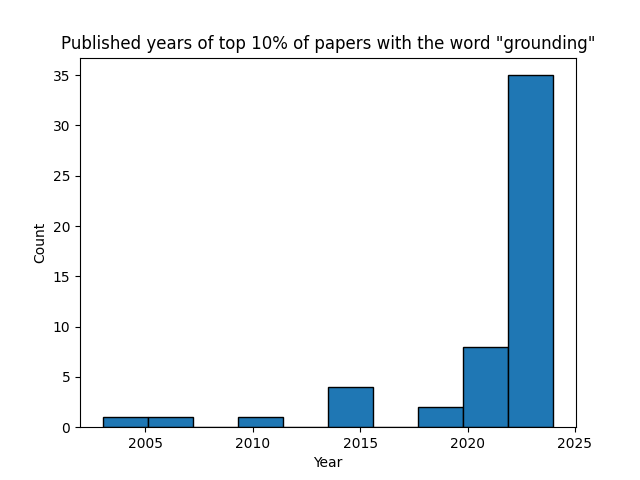
\includegraphics[width=\columnwidth]{figs/years_histogram.png}
  \caption{Count of selected conference papers per year}
  \label{fig:conference_years}
\end{figure}

\section{Grounding ``grounding''}
In this section we cover the 8 different senses of the word ``grounding'' found in the 46 papers covered in the previous section. We will explore the meanings of each sense and the challenges that each paper is tackling. The delineation of these different senses tend to be ambiguous; understanding whether certain senses belong to certain categories can be argued. Rather, categories were chosen according to modality and how differently ``grounding'' would be utilized and established.

\subsection{Visual Grounding}
\label{sec:visual}
Visual grounding, also known as image, phrase or referring expression grounding \cite{xiao2024visualgroundingsurvey, li-etal-2024-groundinggpt,ma2020learninggenerategroundedvisual,Islam_Gladstone_Iqbal_2023_PATRON, jiang-etal-2019-tiger,lu-etal-2022-extending, dou-peng-2021-improving,surikuchi-etal-2023-groovist} refers to the challenge of trying to localize specific regions within an image based on some textual description\footnote{other terms include natural language object retrieval or phrase localization \cite{gigapixel}}. Traditionally, this involved finding the phrase's referring region by predicting a bounding box around said region. As time has gone on however, there has been more and more types of challenges that one could tackle within visual grounding \cite{xiao2024visualgroundingsurvey}. From the 46 papers we filtered for, we have discovered the following subcategories involved in visual grounding.

\subsubsection{Classical Visual Grounding}
This entails the traditional problem of trying to predict a bounding box around a region \cite{li-etal-2024-groundinggpt,huang2021deconfoundedvisualgrounding,peng2023kosmos2groundingmultimodallarge}. Recent papers have found different methods in an attempt to improve performance.  \citet{Zeng_2024_CVPR_Comp_Challenge} improves compositional understanding through providing a harder dataset that relies on introducing different compositions of objects. \citet{neurips_zhang_contrastive_learning} improves performance in weakly supervised (no bounding box annotations) settings through contrastive learning. \citet{gigapixel} provides a new dataset for higher resolution images at different granularity and bounding box sizes. \citet{lee2024regroundimprovingtextualspatial} has shown improvements in image generation as well.

This visual grounding task can be understood as the inverse problem to image captioning, where one is given an image and need to provide the text portion. In fact, this inverse paradigm has led to better models \cite{wang2023cycleconsistencylearningcaptioninggrounding} involving cyclic updates.

\subsubsection{Answer Grounding}
Rather than fit a bounding box to various objects, Visual Question Answering (VQA) grounding attempts to find specific parts of an image that corresponds with inputted questions rather than descriptive prompts \cite{chen2022groundinganswersvisualquestions, Chen_2023_ICCV_vqa}.

\subsection{Action Grounding}
\label{sec:action}
Relying on other types of grounding such as image grounding, action grounding is a term that refers to building a model that is able to take some grounding and relate it to a set of actions. Recent works utilize LLMs in the fields of chat agents, web agents and robotics \cite{zhang2023llavagroundinggroundedvisualchat, cheng-etal-2024-seeclick,zheng2024gpt4visiongeneralistwebagent,Tellex_Kollar_Dickerson_Walter_Banerjee_Teller_Roy_2011_robotic_navigation,wang2023programmaticallygroundedcompositionallygeneralizable} to motivate better actions that are aligned with people's understanding of the world.

Contrary to using image grounding, \citet{kameko-etal-2015-symbol} matches certain states of games to commentary in an attempt to understand how various actions are grounded in language or its symbols. They refer to this type of grounding as ``symbol grounding'' but essentially attempts to relate some action to some other observation.

\subsection{Audio Grounding}
\label{sec:audio}
Audio grounding is the task of taking static images and sounds and attempting to identify which parts of the image are correlated with certain parts of audio. For example, \citet{Tian_2021_CVPR_cyclic_audio} attempts to separate images of bands into which instruments produce what kinds of audio.

\subsection{Video Grounding}
\label{sec:video}
Another related grounding task to visual grounding is the idea of video grounding or spatio-temporal grounding. This task is to identify various portions of a video or the entities within them to provide an understanding for a certain prompt \cite{Jiang_Cheng_Liu_Fang_Peng_Liu_2024_comprehensive_visual_grounding}. These different grounding tasks can be split into its own categories defined in the next sections.

\subsubsection{Object Tracking}
Object tracking relies on the idea that given some natural language prompt, to both identify the specific object within the video but also to continuously track it throughout the video or still frames \cite{Zhou_2023_CVPR_Tracking}.

\subsubsection{Natural Language Spatial Video Grounding}
This video grounding task is an extension of classic visual grounding, where the model attempts to set a bounding box for each frame of a video \cite{li-etal-2022-end-to-end-information-tree,ma2020learninggenerategroundedvisual}.

\subsubsection{Temporal Video Grounding}
This video grounding task is to identify the timestamps in which a prompt holds true for a video \cite{li-etal-2024-groundinggpt, NEURIPS2023_how_to_video,Bao_Zheng_Mu_2021_dense_events, chen-etal-2018-temporally}.

\subsubsection{Spatio-temporal Video Grounding}
This video grounding task combines the last two tasks and attempts to identify both the bounding boxes and the timestamps in which a prompt holds true for a video \cite{Wasim_2024_CVPR_DINO,Chen_2024_CVPR_self_supervised_spatio_temporal,jin2022embracingconsistencyonestageapproach}. It can be used within various settings including video entailment which determines whether a prompt holds true for some video \cite{Chen_2021_ICCV_video_entailment}. Similar to image grounding, video grounding can also be used within video generation tools \cite{jeong2024groundavideozeroshotgroundedvideo}.

\subsection{3D Grounding}
\label{sec:3d}
Similar to image grounding, 3D grounding adds a dimension and attempts to put bounding boxes around 3D models which are often represented as point clouds. These 3D grounding tasks share similar strategies to image grounding, using captioning tasks to improve performance \cite{Cai_2022_CVPR_3DJCG,NEURIPS2023_exploiting_context_3d, NEURIPS2023_city_refer_3d,wang20233drpnet3drelativepositionaware}. Some papers have even used 2D object representations to improve 3D grounding \cite{Yang_2021_ICCV_sat_2d}, while others have improved 3D visual grounding with reasoning \cite{zhu2024scanreasonempowering3dvisual}.

\subsection{Dialogue Grounding}
\label{sec:dialogue}
This term of ``dialogue grounding'' is loosely defined, usually seen in literature simply as ``grounding''. Within these papers, ``grounding'' refers to the idea of trying to build a common ground of understanding between two or more actors within a conversation. It includes attempting to analyze nonverbal behaviours \cite{nakano-etal-2003-towards,Roque2007ReactingTA_dialogue, liu-etal-2012-towards,shaikh2024groundinggapslanguagemodel}.

\subsection{Markov Logic Networks Grounding}
\label{sec:markov}
``Grounding'' in Markov Logic Networks (MLNs) differs significantly from the other senses of the word \cite{NIPS2014_markov_logic_networks}. MLNs refer to a statistical model for probabilistic logic reasoning, where by developing a set of first-order logic rules known as ``grounds'' one is able to form a weighted satisfiability problem with an optimized solution. In particular, grounding within Markov Logic Networks refers to the process of forming the weighted satisfiability graph \cite{MLN4KB_markov}.

\subsection{Physical Dynamics Grounding}
\label{sec:dynamics}
Attempting to model physical dynamics purely from states and its transitions tend to be difficult, requiring a ton of resources to supervise consecutive particle properties. Instead of requiring this supervision, a new field has emerged to attempt to understand these physical dynamics from visual observations \cite{NEURIPS2024_neuma_material_visual_grounding}. One such application is in fluid dynamics grounding; which attempts to build an understanding of fluid particle systems from sequential visual observations \cite{guan2022neurofluidfluiddynamicsgrounding}. 

\section{Analyzing ``grounding'''s Usage}
In this section, we will build a quantitative understanding of ``grounding'' and its senses over time. We will explore how the word has been used throughout the years, and dive deeper into a few senses of the word. We will accomplish this through observing the co-occurrence trends over time with other key words for each specific sense.

\subsection{``grounding'' Over Time}
In this section, we explore how the term ``grounding'' has evolved over time through analyzing how many papers have included the term ``grounding''. We aggregate over all the data splits while showcasing a more fine-grained example for a specific conference to avoid any patterns lost through aggregation.

In particular, we observe that the number of instances of ``grounding'' has increased both in terms of pure count and frequency over time (see Fig~\ref{fig:all_confs_count} and Fig~\ref{fig:all_confs_freq}). We normalize because the number of papers being published in general increases as well, naturally inflating the number of ``grounding'' papers. However we observe that both the pure count and frequency increase over time, concluding that ``grounding'' has been a terminology that is becoming more and more utilized. This is likely due to it becoming more relevant with the uprise of multimodal models \cite{xiao2024visualgroundingsurvey} and a need to interpret and improve these models.

\begin{figure}[h]
  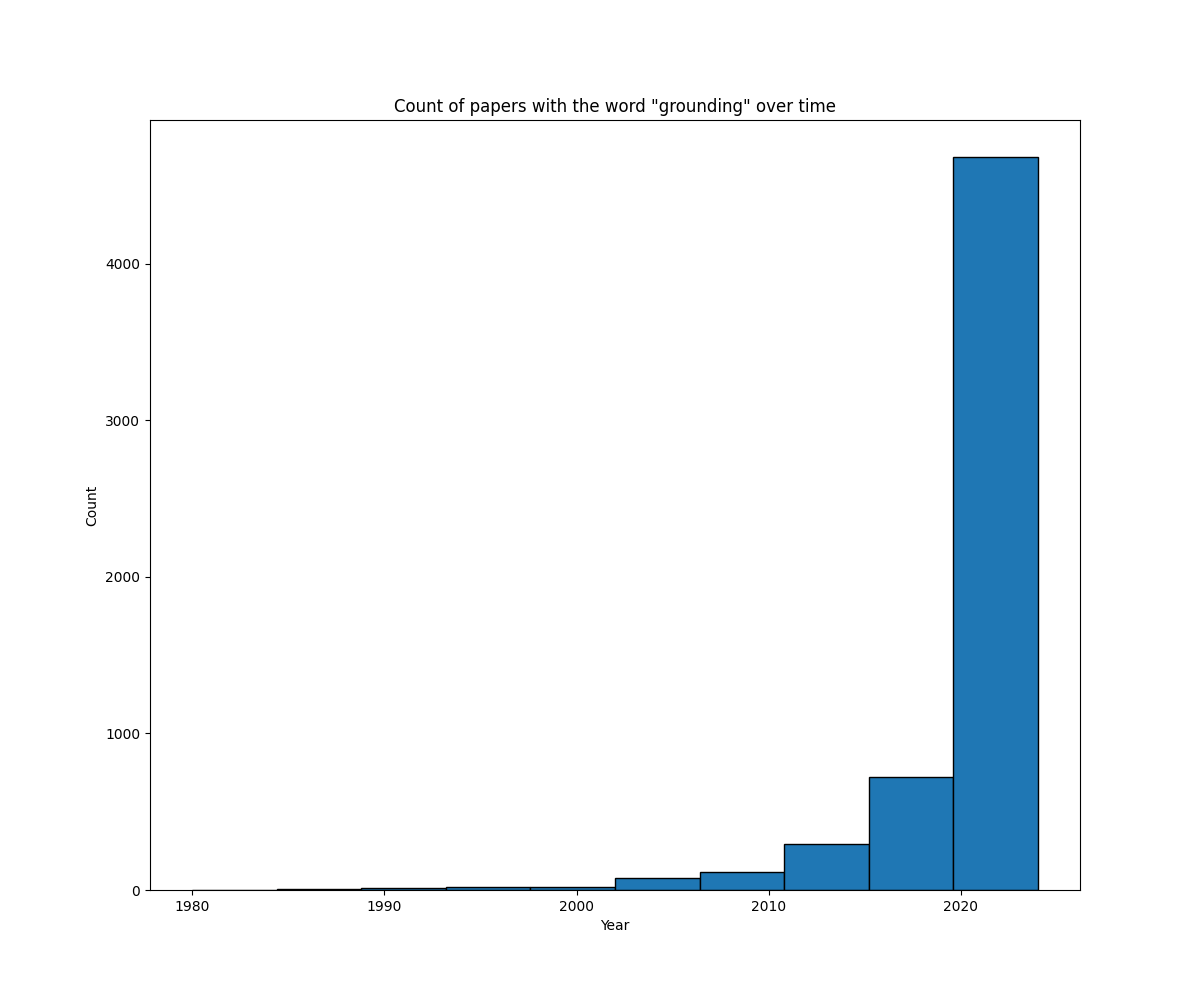
\includegraphics[width=\columnwidth]{figs/year_distribution/all_confs_grounding.png}
  \caption{Count of ``grounding'' for all the conferences over time}
  \label{fig:all_confs_count}
\end{figure}

\begin{figure}[h]
  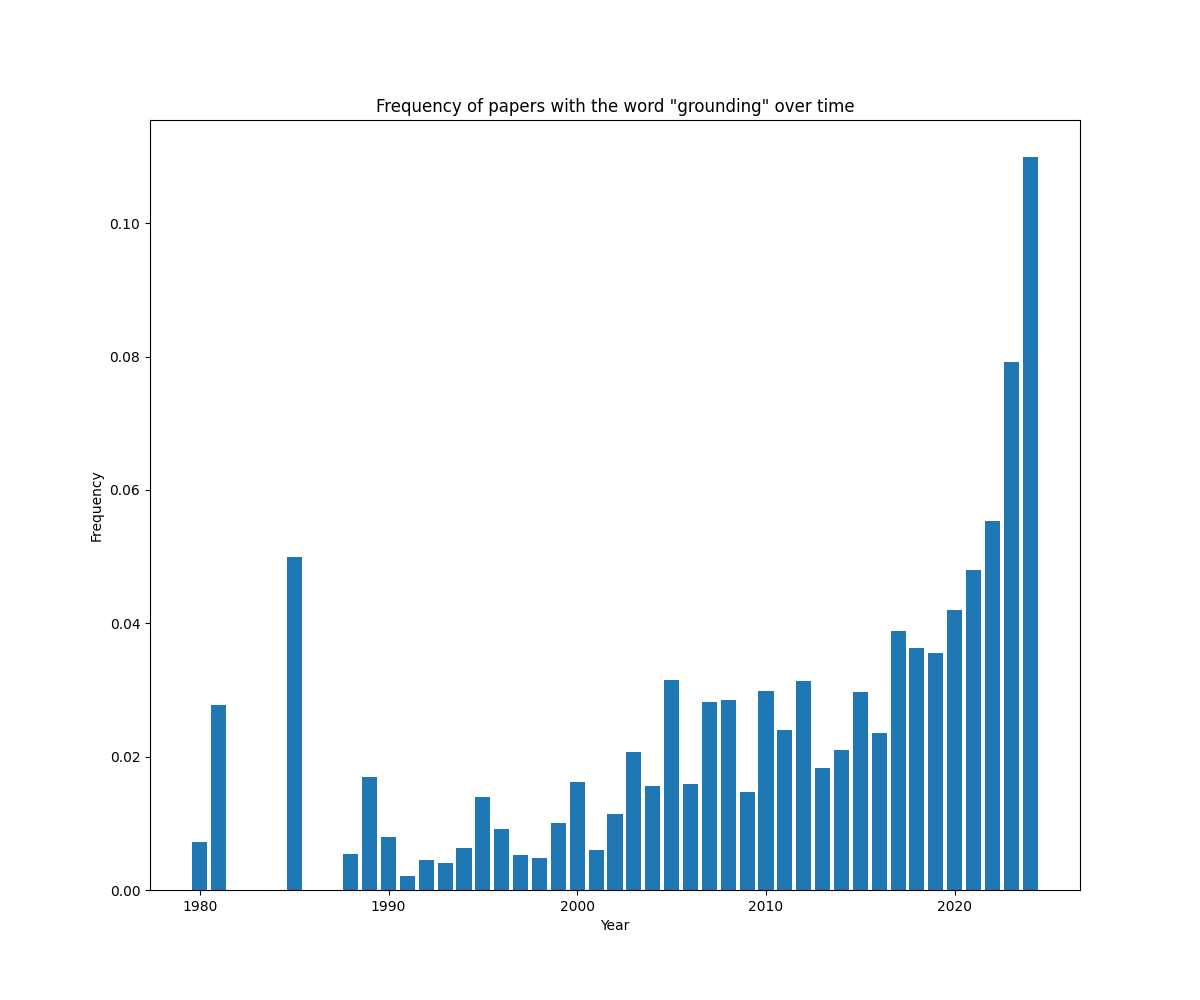
\includegraphics[width=\columnwidth]{figs/year_distribution_freq/all_confs_grounding_dist.png}
  \caption{Frequency of papers containing the word ``grounding'' for all conferences over time}
  \label{fig:all_confs_freq}
\end{figure}

To see how each individual conference's count and frequency changes over time, see Appendix~\ref{sec:appendix_years}. These graphs do confirm that our selection of papers in the previous section were well-justified, as the most important papers relevant to ``grounding'' are likely to be the more recent papers. Therefore, not having covered senses of ``grounding'' from papers spanning the 1980's-2000's is not as significant as it may seem.

\subsection{``grounding'' Senses Over Time}
\label{sec:coocurrence}
We observed that the different senses of the word ``grounding'' are not uniformly distributed across time, rather that it has evolved. Take ``dialogue grounding'', where our filtered papers were some of the only ones from the 2000s \cite{nakano-etal-2003-towards,Roque2007ReactingTA_dialogue} with more recent papers covering other senses of the word. To better understand ``grounding'''s evolution, this section here covers different word co-occurrences over time.

In particular, we explore the frequency of papers that include the word ``grounding'' which also contains other words which can indicate different senses. Table~\ref{tab:word_senses} in Appendix~\ref{sec:appendix_word_matching} shows which words we count as co-occuring for each sense. In the following sections we explore how these co-occurrences change over time.

\subsubsection{Visual Grounding}
For visual grounding, we can tell that only more recently has there been an increase in the number of papers dealing with the visual grounding paradigm. According to \citet{xiao2024visualgroundingsurvey}, this is likely due to improvements in multimodal models in 2021, correlating with our findings in Fig~\ref{fig:visual_all_confs_count} and Fig~\ref{fig:visual_all_confs_freq}.

\begin{figure}[h!]
  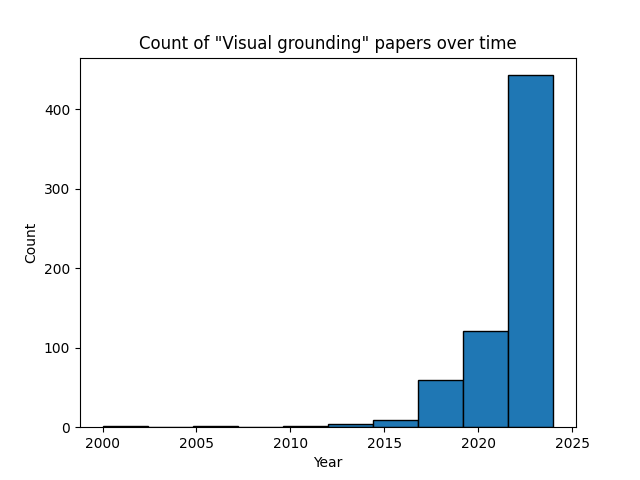
\includegraphics[width=\columnwidth]{figs/grounding_figs/Visual/all_confs_grounding_Visual.png}
  \caption{Count of ``visual grounding'' for all the conferences over time}
  \label{fig:visual_all_confs_count}
\end{figure}

\begin{figure}[h!]
  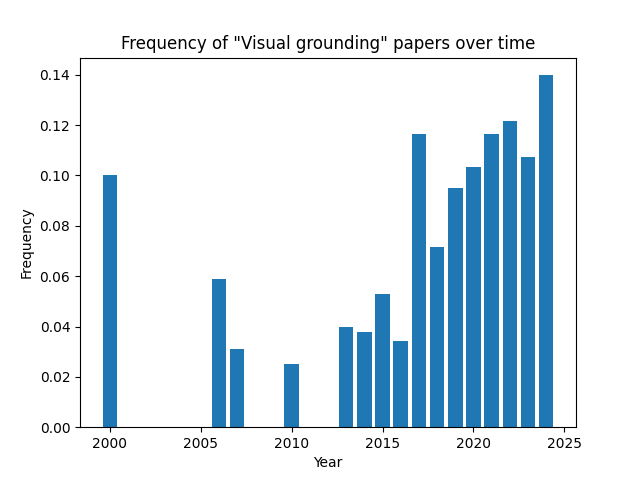
\includegraphics[width=\columnwidth]{figs/freq_grounding_figs/Visual/all_confs_grounding_Visual.png}
  \caption{Frequency of ``visual grounding'' for all conferences over time}
  \label{fig:visual_all_confs_freq}
\end{figure}

See Appendix~\ref{sec:appendix_word_sense_years_visual_grounding} for the splits per conference.

\subsubsection{Action Grounding}
For action grounding, there has been a steady interest over time shown by the frequency of papers which sit around 50\%. At first glance, this seems high and likely to be conflated due to search words such as ``web'' or ``agent''. However, as action grounding refers to the applicability of other types of grounding this is likely representative of the word sense itself.

A noteable observation is that the frequency of ``grounding'' papers in earlier years such as within the 1990s tend to have very high frequency that matches with ``action grounding''. This is likely due to the small sample size within those time periods, having only AAAI, ACL, IJCAI and NeurIPS as conferences, each with a small magnitude of publications. This reduces the variability and thus we would expect to see higher frequencies of certain senses of words during these time periods. This trend follows for the other senses.
\begin{figure}[h!]
  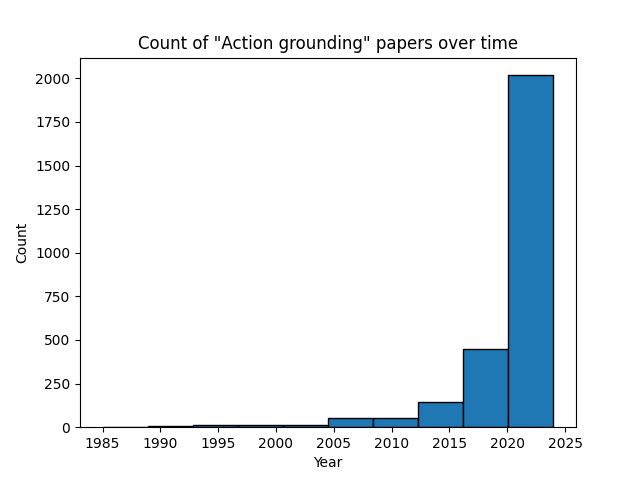
\includegraphics[width=\columnwidth]{figs/grounding_figs/Action/all_confs_grounding_Action.png}
  \caption{Count of ``Action grounding'' for all the conferences over time}
  \label{fig:action_all_confs_count}
\end{figure}

\begin{figure}[h!]
  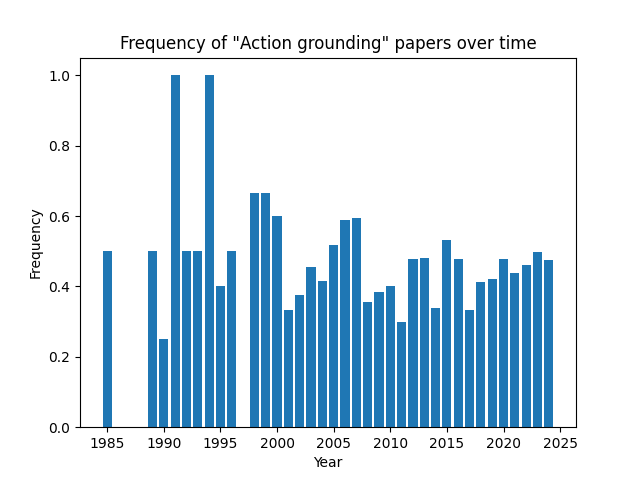
\includegraphics[width=\columnwidth]{figs/freq_grounding_figs/Action/all_confs_grounding_Action.png}
  \caption{Frequency of ``Action grounding'' for all conferences over time}
  \label{fig:action_all_confs_freq}
\end{figure}

See Appendix~\ref{sec:appendix_word_sense_years_action} for the splits per conference.

\subsubsection{Audio Grounding}
There seems to be less papers revolved around audio grounding, as after the 2000s, it is at most referenced in about 20\% of the papers. Even as the multimodal model mark in 2021 hits, there has been a slight increase but still smaller share of the ``grounding'' papers count.
\begin{figure}[h!]
  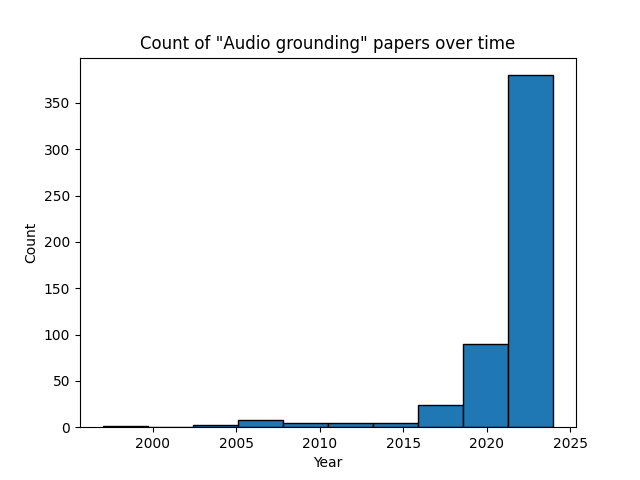
\includegraphics[width=\columnwidth]{figs/grounding_figs/Audio/all_confs_grounding_Audio.png}
  \caption{Count of ``Audio grounding'' for all the conferences over time}
  \label{fig:audio_all_confs_count}
\end{figure}

\begin{figure}[h!]
  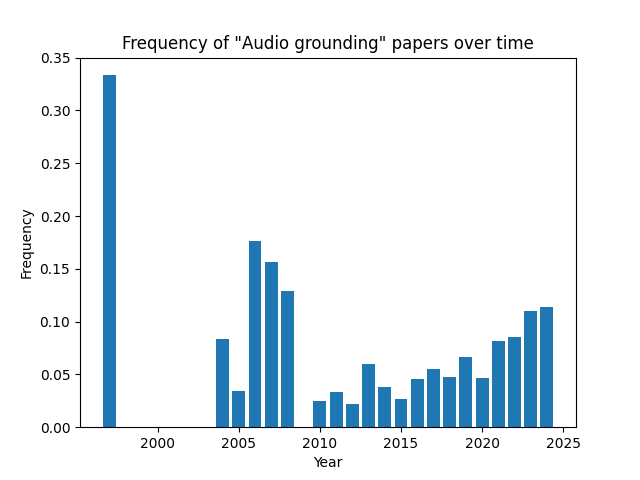
\includegraphics[width=\columnwidth]{figs/freq_grounding_figs/Audio/all_confs_grounding_Audio.png}
  \caption{Frequency of ``Audio grounding'' for all conferences over time}
  \label{fig:audio_all_confs_freq}
\end{figure}

See Appendix~\ref{sec:appendix_word_sense_years_audio} for the splits per conference.

\subsubsection{Video Grounding}
After the 2000s, the video grounding sense follows a very similar trend to audio grounding, but with a significantly higher share at around 50-60\% of papers. This is likely due to the fact that most multimodal models that work on video also work on other senses of grounding such as audio and image grounding \cite{li-etal-2024-groundinggpt}.
\begin{figure}[h!]
  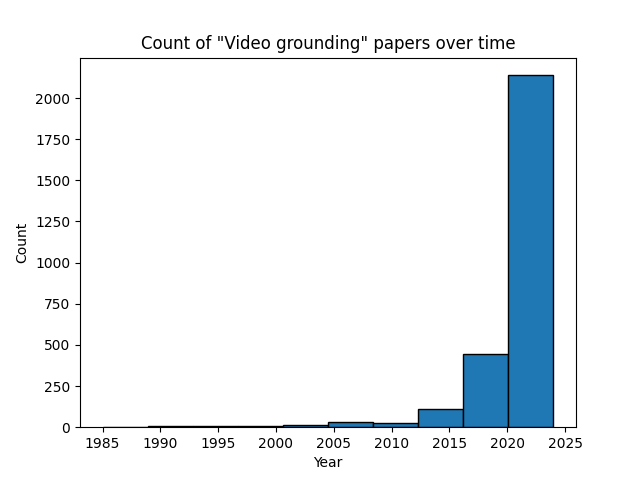
\includegraphics[width=\columnwidth]{figs/grounding_figs/Video/all_confs_grounding_Video.png}
  \caption{Count of ``Video grounding'' for all the conferences over time}
  \label{fig:video_all_confs_count}
\end{figure}

\begin{figure}[h!]
  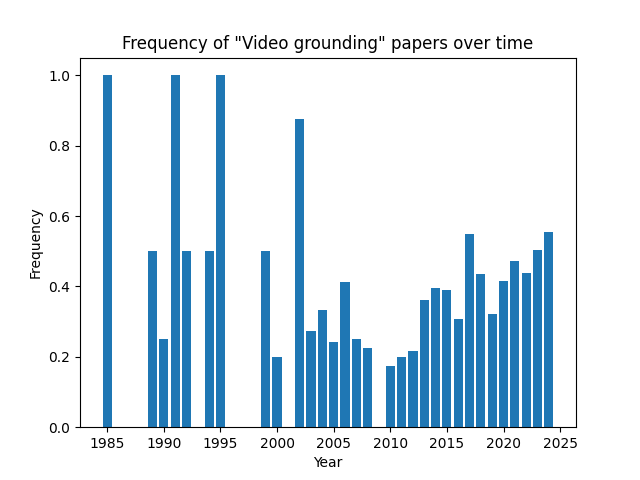
\includegraphics[width=\columnwidth]{figs/freq_grounding_figs/Video/all_confs_grounding_Video.png}
  \caption{Frequency of ``Video grounding'' for all conferences over time}
  \label{fig:video_all_confs_freq}
\end{figure}

See Appendix~\ref{sec:appendix_word_sense_years_video} for the splits per conference.

\subsubsection{3D Grounding}
3D grounding observes a huge spike in papers around the 2020s, likely due to significant advancements in marquee papers such as ScanRefer \cite{chen2020scanrefer3dobjectlocalization,liu2024surveytextguided3dvisual}. Such papers introduce novel problems which encourages future development and a larger share of the paper frequencies.
\begin{figure}[h!]
  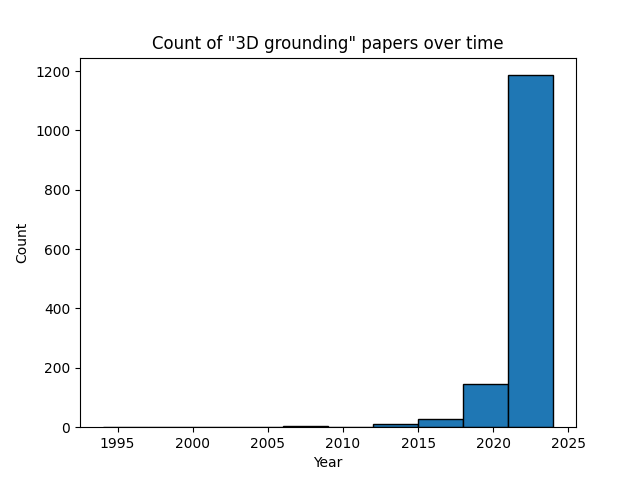
\includegraphics[width=\columnwidth]{figs/grounding_figs/3D/all_confs_grounding_3D.png}
  \caption{Count of ``3D grounding'' for all the conferences over time}
  \label{fig:3d_all_confs_count}
\end{figure}

\begin{figure}[h!]
  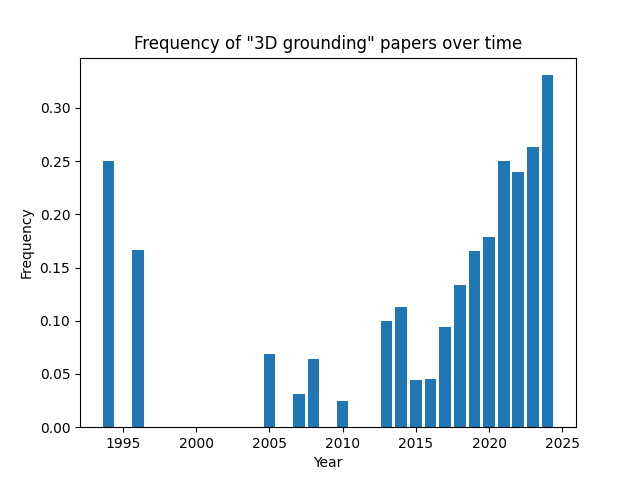
\includegraphics[width=\columnwidth]{figs/freq_grounding_figs/3D/all_confs_grounding_3D.png}
  \caption{Frequency of ``3D grounding'' for all conferences over time}
  \label{fig:3d_all_confs_freq}
\end{figure}

See Appendix~\ref{sec:appendix_word_sense_years_3d} for the splits per conference.

\subsubsection{Dialogue Grounding}
Dialogue grounding's trend follows our empirical observations, where they had a much larger share of papers earlier on in the 2000s, but has since decreased significantly.
\begin{figure}[h!]
  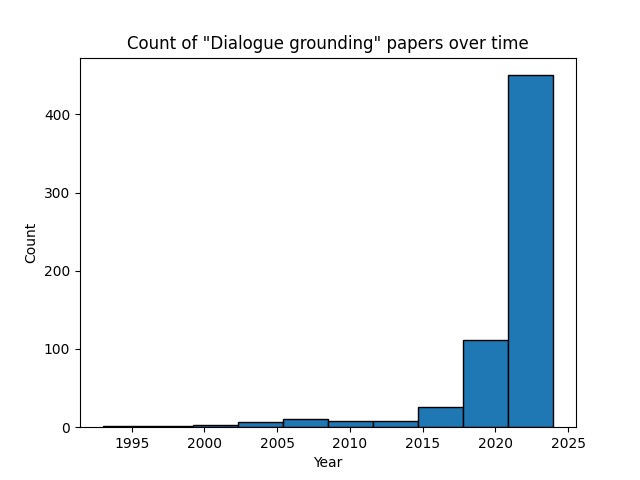
\includegraphics[width=\columnwidth]{figs/grounding_figs/Dialogue/all_confs_grounding_Dialogue.png}
  \caption{Count of ``Dialogue grounding'' for all the conferences over time}
  \label{fig:dialogue_all_confs_count}
\end{figure}

\begin{figure}[h!]
  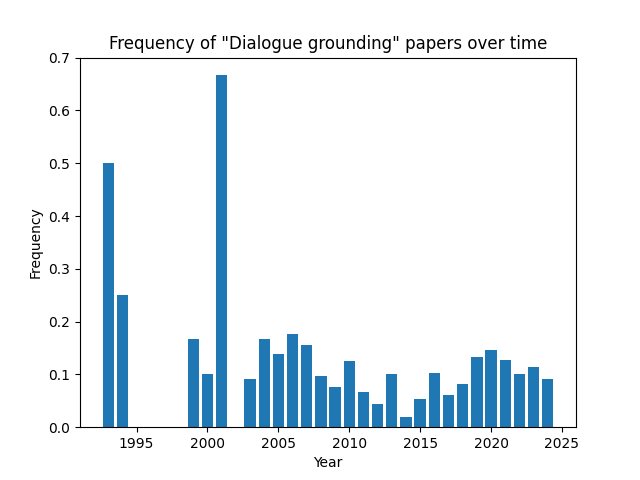
\includegraphics[width=\columnwidth]{figs/freq_grounding_figs/Dialogue/all_confs_grounding_Dialogue.png}
  \caption{Frequency of ``Dialogue grounding'' for all conferences over time}
  \label{fig:dialogue_all_confs_freq}
\end{figure}

See Appendix~\ref{sec:appendix_word_sense_years_dialogue} for the splits per conference.

\subsubsection{Markov Logic Networks Grounding}
Markov Logic Networks were seemingly popular within the 2010s, having a high share of the market at that time. However, as 2020s approached, there seems to be a shift away from Markov probabilistic models and more towards LLMs and multimodal models.

\begin{figure}[h!]
  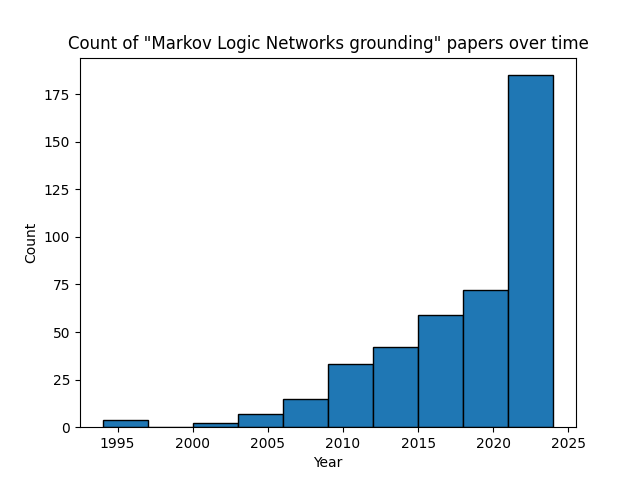
\includegraphics[width=\columnwidth]{figs/grounding_figs/Markov Logic Networks/all_confs_grounding_Markov Logic Networks.png}
  \caption{Count of ``Markov Logic Networks grounding'' for all the conferences over time}
  \label{fig:markov_all_confs_count}
\end{figure}

\begin{figure}[h!]
  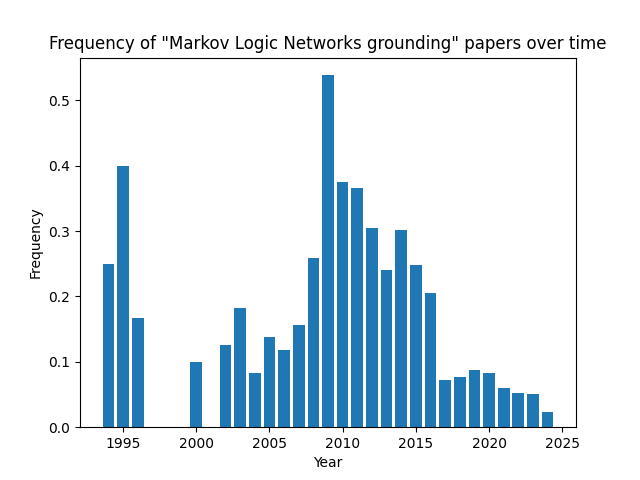
\includegraphics[width=\columnwidth]{figs/freq_grounding_figs/Markov Logic Networks/all_confs_grounding_Markov Logic Networks.png}
  \caption{Frequency of ``Markov Logic Networks grounding'' for all conferences over time}
  \label{fig:markov_all_confs_freq}
\end{figure}

See Appendix~\ref{sec:appendix_word_sense_years_markov} for the splits per conference.

\subsubsection{Physical Dynamics Grounding}
Physical dynamics models tend to be quite niche, leading to a very small share of the amount of papers which include that sense of the word.

\begin{figure}[h!]
  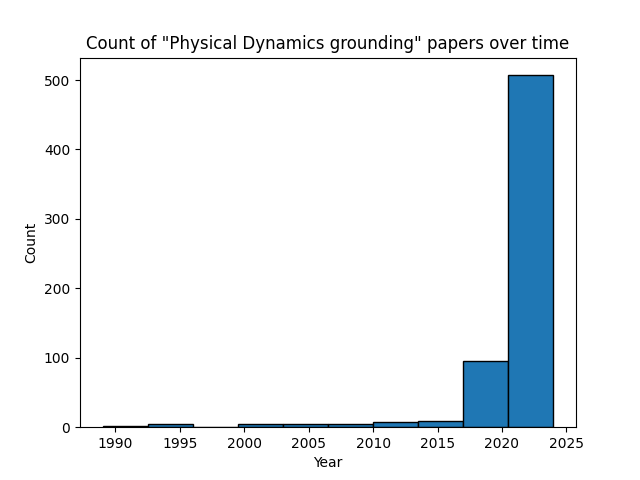
\includegraphics[width=\columnwidth]{figs/grounding_figs/Physical Dynamics/all_confs_grounding_Physical Dynamics.png}
  \caption{Count of ``Physical Dynamics grounding'' for all the conferences over time}
  \label{fig:dynamics_all_confs_count}
\end{figure}

\begin{figure}[h!]
  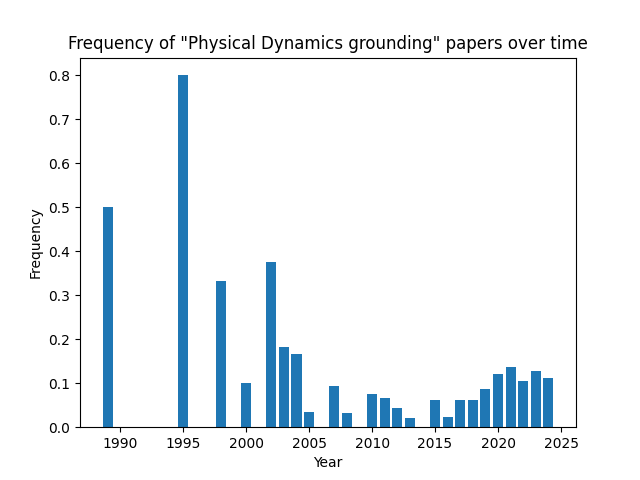
\includegraphics[width=\columnwidth]{figs/freq_grounding_figs/Physical Dynamics/all_confs_grounding_Physical Dynamics.png}
  \caption{Frequency of ``Physical Dynamics grounding'' for all conferences over time}
  \label{fig:dynamics_all_confs_freq}
\end{figure}

See Appendix~\ref{sec:appendix_word_sense_years_dynamics} for the splits per conference.


\section{Conclusion}
This work has shown that ``grounding'' is an overloaded term with many different senses and modalities. These senses have evolved over time, inflating and contracting according to research trends.

In future work, we hope to explore more meta-analysis through quantitative analysis of the different datasets, methods and metrics of each sense. Especially as deep learning and multimodal models become more and more popular, understanding which of these datasets are being the most benchmarked could provide some more insight than a typical survey paper. We also hope to perform more fine-grained meta-analysis, understanding how much of each sense is composed of smaller sub-categories, such as understanding how much of ``action grounding'' is for robotics applications. Furthermore, certain word senses are also ambiguous for its high frequency and nature of encompassing other types of grounding such as ``video grounding''. Future analysis is required to provide a deeper understanding of these dynamics.

% \section{Engines}

% To produce a PDF file, pdf\LaTeX{} is strongly recommended (over original \LaTeX{} plus dvips+ps2pdf or dvipdf).
% The style file \texttt{acl.sty} can also be used with
% lua\LaTeX{} and
% Xe\LaTeX{}, which are especially suitable for text in non-Latin scripts.
% The file \texttt{acl\_lualatex.tex} in this repository provides
% an example of how to use \texttt{acl.sty} with either
% lua\LaTeX{} or
% Xe\LaTeX{}.

% \section{Preamble}

% The first line of the file must be
% \begin{quote}
% \begin{verbatim}
% \documentclass[11pt]{article}
% \end{verbatim}
% \end{quote}

% To load the style file in the review version:
% \begin{quote}
% \begin{verbatim}
% \usepackage[review]{acl}
% \end{verbatim}
% \end{quote}
% For the final version, omit the \verb|review| option:
% \begin{quote}
% \begin{verbatim}
% \usepackage{acl}
% \end{verbatim}
% \end{quote}

% To use Times Roman, put the following in the preamble:
% \begin{quote}
% \begin{verbatim}
% \usepackage{times}
% \end{verbatim}
% \end{quote}
% (Alternatives like txfonts or newtx are also acceptable.)

% Please see the \LaTeX{} source of this document for comments on other packages that may be useful.

% Set the title and author using \verb|\title| and \verb|\author|. Within the author list, format multiple authors using \verb|\and| and \verb|\And| and \verb|\AND|; please see the \LaTeX{} source for examples.

% By default, the box containing the title and author names is set to the minimum of 5 cm. If you need more space, include the following in the preamble:
% \begin{quote}
% \begin{verbatim}
% \setlength\titlebox{<dim>}
% \end{verbatim}
% \end{quote}
% where \verb|<dim>| is replaced with a length. Do not set this length smaller than 5 cm.

% \section{Document Body}

% \subsection{Footnotes}

% Footnotes are inserted with the \verb|\footnote| command.\footnote{This is a footnote.}

% \subsection{Tables and figures}

% See Table~\ref{tab:accents} for an example of a table and its caption.
% \textbf{Do not override the default caption sizes.}

% \begin{table}
%   \centering
%   \begin{tabular}{lc}
%     \hline
%     \textbf{Command} & \textbf{Output} \\
%     \hline
%     \verb|{\"a}|     & {\"a}           \\
%     \verb|{\^e}|     & {\^e}           \\
%     \verb|{\`i}|     & {\`i}           \\
%     \verb|{\.I}|     & {\.I}           \\
%     \verb|{\o}|      & {\o}            \\
%     \verb|{\'u}|     & {\'u}           \\
%     \verb|{\aa}|     & {\aa}           \\\hline
%   \end{tabular}
%   \begin{tabular}{lc}
%     \hline
%     \textbf{Command} & \textbf{Output} \\
%     \hline
%     \verb|{\c c}|    & {\c c}          \\
%     \verb|{\u g}|    & {\u g}          \\
%     \verb|{\l}|      & {\l}            \\
%     \verb|{\~n}|     & {\~n}           \\
%     \verb|{\H o}|    & {\H o}          \\
%     \verb|{\v r}|    & {\v r}          \\
%     \verb|{\ss}|     & {\ss}           \\
%     \hline
%   \end{tabular}
%   \caption{Example commands for accented characters, to be used in, \emph{e.g.}, Bib\TeX{} entries.}
%   \label{tab:accents}
% \end{table}

% As much as possible, fonts in figures should conform
% to the document fonts. See Figure~\ref{fig:experiments} for an example of a figure and its caption.

% Using the \verb|graphicx| package graphics files can be included within figure
% environment at an appropriate point within the text.
% The \verb|graphicx| package supports various optional arguments to control the
% appearance of the figure.
% You must include it explicitly in the \LaTeX{} preamble (after the
% \verb|\documentclass| declaration and before \verb|\begin{document}|) using
% \verb|\usepackage{graphicx}|.

% \begin{figure}[t]
%   \includegraphics[width=\columnwidth]{example-image-golden}
%   \caption{A figure with a caption that runs for more than one line.
%     Example image is usually available through the \texttt{mwe} package
%     without even mentioning it in the preamble.}
%   \label{fig:experiments}
% \end{figure}

% \begin{figure*}[t]
%   \includegraphics[width=0.48\linewidth]{example-image-a} \hfill
%   \includegraphics[width=0.48\linewidth]{example-image-b}
%   \caption {A minimal working example to demonstrate how to place
%     two images side-by-side.}
% \end{figure*}

% \subsection{Hyperlinks}

% Users of older versions of \LaTeX{} may encounter the following error during compilation:
% \begin{quote}
% \verb|\pdfendlink| ended up in different nesting level than \verb|\pdfstartlink|.
% \end{quote}
% This happens when pdf\LaTeX{} is used and a citation splits across a page boundary. The best way to fix this is to upgrade \LaTeX{} to 2018-12-01 or later.

% \subsection{Citations}

% \begin{table*}
%   \centering
%   \begin{tabular}{lll}
%     \hline
%     \textbf{Output}           & \textbf{natbib command} & \textbf{ACL only command} \\
%     \hline
%     \citep{Gusfield:97}       & \verb|\citep|           &                           \\
%     \citealp{Gusfield:97}     & \verb|\citealp|         &                           \\
%     \citet{Gusfield:97}       & \verb|\citet|           &                           \\
%     \citeyearpar{Gusfield:97} & \verb|\citeyearpar|     &                           \\
%     \citeposs{Gusfield:97}    &                         & \verb|\citeposs|          \\
%     \hline
%   \end{tabular}
%   \caption{\label{citation-guide}
%     Citation commands supported by the style file.
%     The style is based on the natbib package and supports all natbib citation commands.
%     It also supports commands defined in previous ACL style files for compatibility.
%   }
% \end{table*}

% Table~\ref{citation-guide} shows the syntax supported by the style files.
% We encourage you to use the natbib styles.
% You can use the command \verb|\citet| (cite in text) to get ``author (year)'' citations, like this citation to a paper by \citet{Gusfield:97}.
% You can use the command \verb|\citep| (cite in parentheses) to get ``(author, year)'' citations \citep{Gusfield:97}.
% You can use the command \verb|\citealp| (alternative cite without parentheses) to get ``author, year'' citations, which is useful for using citations within parentheses (e.g. \citealp{Gusfield:97}).

% A possessive citation can be made with the command \verb|\citeposs|.
% This is not a standard natbib command, so it is generally not compatible
% with other style files.

% \subsection{References}

% \nocite{Ando2005,andrew2007scalable,rasooli-tetrault-2015}

% The \LaTeX{} and Bib\TeX{} style files provided roughly follow the American Psychological Association format.
% If your own bib file is named \texttt{custom.bib}, then placing the following before any appendices in your \LaTeX{} file will generate the references section for you:
% \begin{quote}
% \begin{verbatim}
% \bibliography{custom}
% \end{verbatim}
% \end{quote}

% You can obtain the complete ACL Anthology as a Bib\TeX{} file from \url{https://aclweb.org/anthology/anthology.bib.gz}.
% To include both the Anthology and your own .bib file, use the following instead of the above.
% \begin{quote}
% \begin{verbatim}
% \bibliography{anthology,custom}
% \end{verbatim}
% \end{quote}

% Please see Section~\ref{sec:bibtex} for information on preparing Bib\TeX{} files.

% \subsection{Equations}

% An example equation is shown below:
% \begin{equation}
%   \label{eq:example}
%   A = \pi r^2
% \end{equation}

% Labels for equation numbers, sections, subsections, figures and tables
% are all defined with the \verb|\label{label}| command and cross references
% to them are made with the \verb|\ref{label}| command.

% This an example cross-reference to Equation~\ref{eq:example}.

% \subsection{Appendices}

% Use \verb|\appendix| before any appendix section to switch the section numbering over to letters. See Appendix~\ref{sec:appendix} for an example.

% \section{Bib\TeX{} Files}
% \label{sec:bibtex}

% Unicode cannot be used in Bib\TeX{} entries, and some ways of typing special characters can disrupt Bib\TeX's alphabetization. The recommended way of typing special characters is shown in Table~\ref{tab:accents}.

% Please ensure that Bib\TeX{} records contain DOIs or URLs when possible, and for all the ACL materials that you reference.
% Use the \verb|doi| field for DOIs and the \verb|url| field for URLs.
% If a Bib\TeX{} entry has a URL or DOI field, the paper title in the references section will appear as a hyperlink to the paper, using the hyperref \LaTeX{} package.

\section*{Limitations}
This section discusses the possible limitations from our selection process and meta-analysis. Regarding our selection process, there is potential bias in choosing the most important 10\% of papers due to the nature of some work being longer with more citations and thus requiring more ``grounding'' occurrences to rank as important. This might lead to some over-representation of senses and a lack of other senses within the filtered papers. Similarly, the most 10\% of papers might be confounded by time, as time goes on, there is an increase in the number of papers and conferences, which might artificially inflate the number of papers with more modern senses.

For our meta-analysis, our selection method of the words chosen might introduce some unwanted bias. In particular, words such as ``sound'' has an ambiguous semantic meaning, either referring to a sound argument or the production of noise. Future works should reduce this limitation by having better filtering in place.

% Since December 2023, a "Limitations" section has been required for all papers submitted to ACL Rolling Review (ARR). This section should be placed at the end of the paper, before the references. The "Limitations" section (along with, optionally, a section for ethical considerations) may be up to one page and will not count toward the final page limit. Note that these files may be used by venues that do not rely on ARR so it is recommended to verify the requirement of a "Limitations" section and other criteria with the venue in question.

% \section*{Acknowledgments}

% This document has been adapted
% by Steven Bethard, Ryan Cotterell and Rui Yan
% from the instructions for earlier ACL and NAACL proceedings, including those for
% ACL 2019 by Douwe Kiela and Ivan Vuli\'{c},
% NAACL 2019 by Stephanie Lukin and Alla Roskovskaya,
% ACL 2018 by Shay Cohen, Kevin Gimpel, and Wei Lu,
% NAACL 2018 by Margaret Mitchell and Stephanie Lukin,
% Bib\TeX{} suggestions for (NA)ACL 2017/2018 from Jason Eisner,
% ACL 2017 by Dan Gildea and Min-Yen Kan,
% NAACL 2017 by Margaret Mitchell,
% ACL 2012 by Maggie Li and Michael White,
% ACL 2010 by Jing-Shin Chang and Philipp Koehn,
% ACL 2008 by Johanna D. Moore, Simone Teufel, James Allan, and Sadaoki Furui,
% ACL 2005 by Hwee Tou Ng and Kemal Oflazer,
% ACL 2002 by Eugene Charniak and Dekang Lin,
% and earlier ACL and EACL formats written by several people, including
% John Chen, Henry S. Thompson and Donald Walker.
% Additional elements were taken from the formatting instructions of the \emph{International Joint Conference on Artificial Intelligence} and the \emph{Conference on Computer Vision and Pattern Recognition}.

% Bibliography entries for the entire Anthology, followed by custom entries
%\bibliography{anthology,custom}
% Custom bibliography entries only
\bibliography{custom}

\onecolumn
\clearpage
\appendix

\section{Distribution of years per conference}
\label{sec:appendix_years}
In Fig~\ref{fig:all_confs_count} and Fig~\ref{fig:all_confs_freq}, we only showed what the aggregated counts and frequency of ``grounding'' over time were, possibly hiding some trends. The following figures showcase that the individual conference trends follow the overall trend of increasing in both count and frequency over time.

\begin{figure*}[h]
  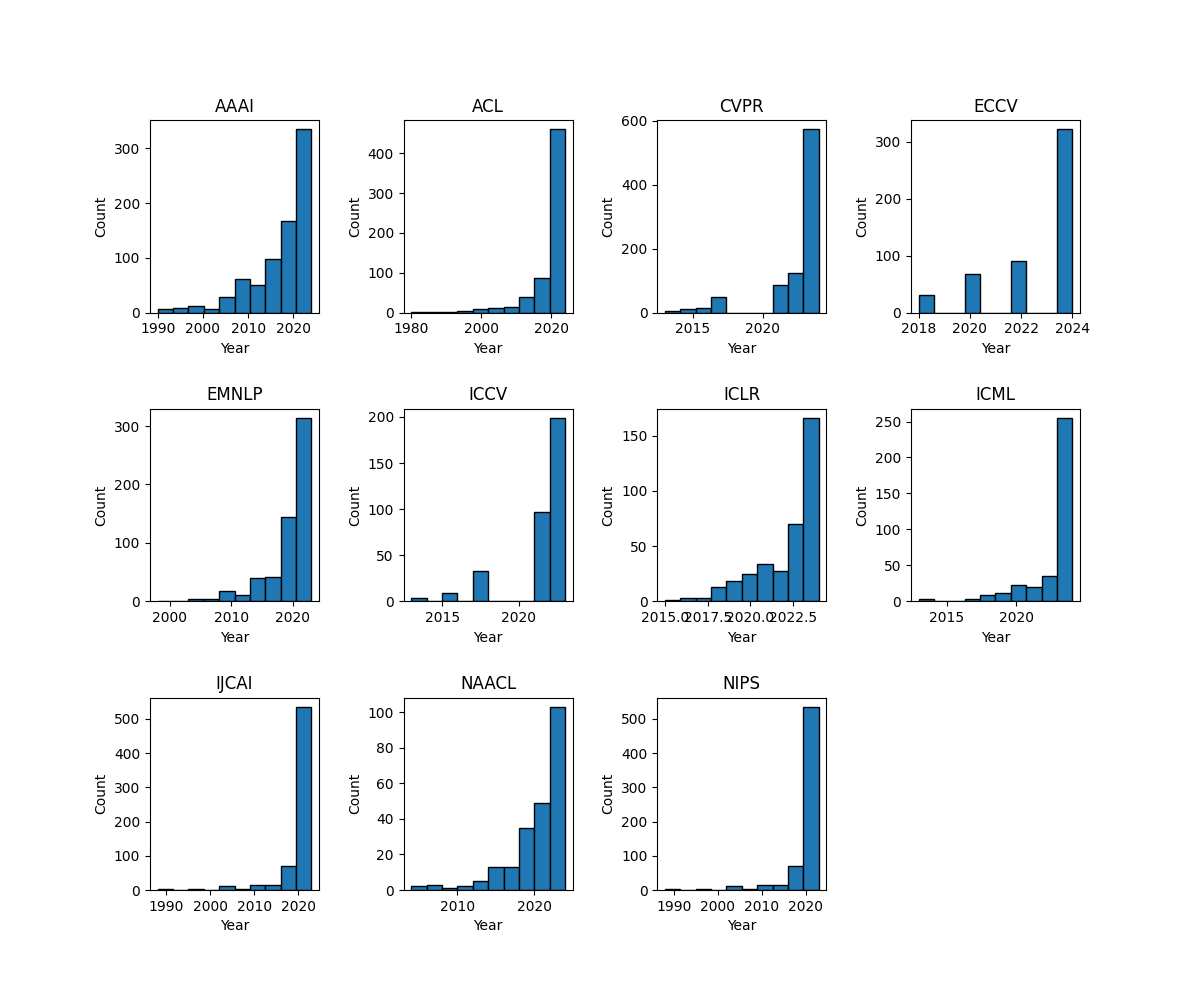
\includegraphics[width=0.6\linewidth]{figs/year_distribution/split_by_conf_grounding_dist.png} 
  \centering
  \caption {Count of ``grounding'' for all conferences over time}
\end{figure*}

\begin{figure*}[h]
  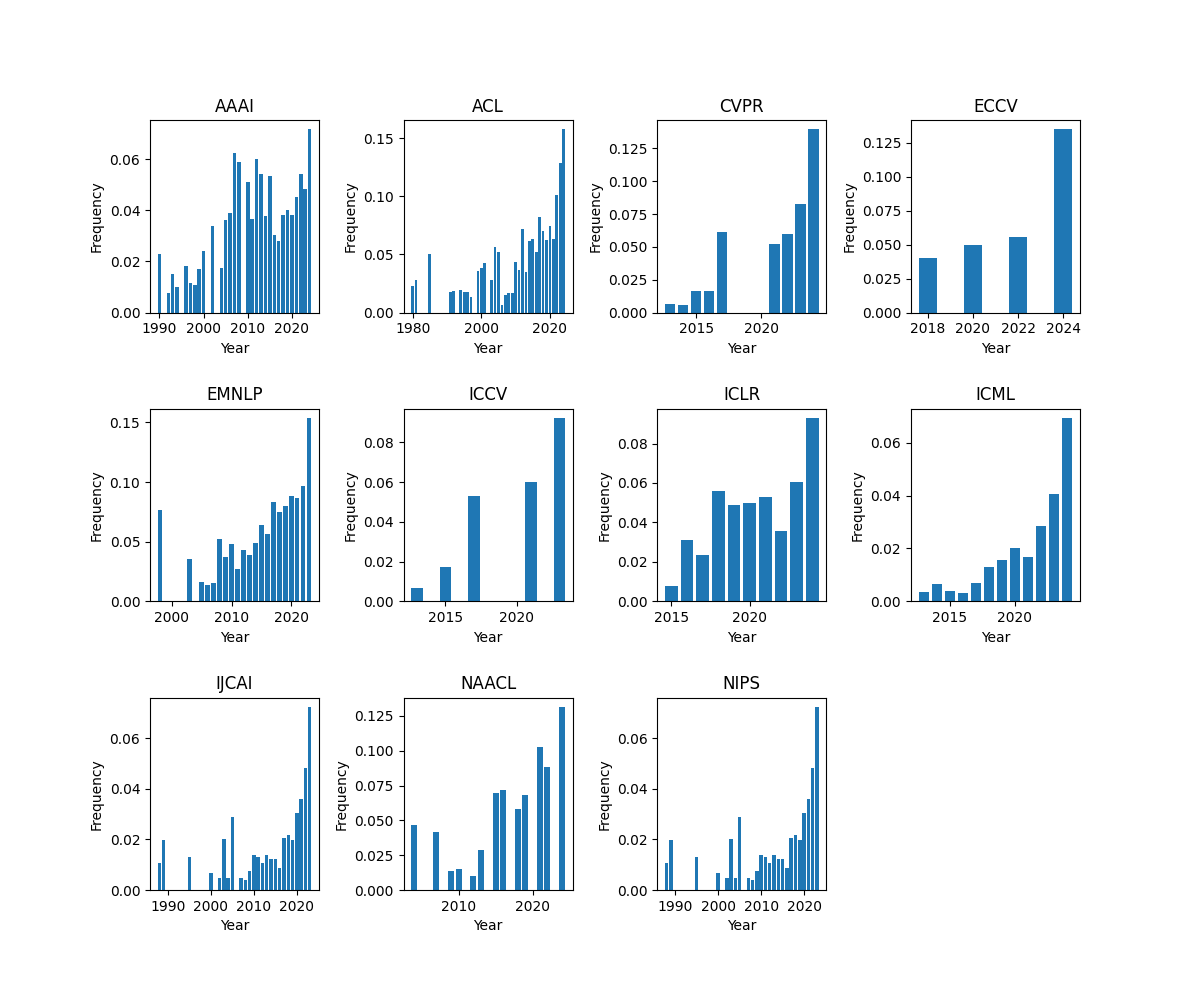
\includegraphics[width=0.6\linewidth]{figs/year_distribution_freq/split_by_conf_grounding_dist.png} 
  \centering
  \caption {Frequency of papers containing the word ``grounding'' for all conferences over time}
\end{figure*}

\clearpage
\section{Words to match per word sense}
\label{sec:appendix_word_matching}

For counting co-occurrences in section~\ref{sec:coocurrence}, we want to pattern match for specific words. In particular, we will match a single word from the list while doing partial matching, and being case insensitive. We ensure that each paper is only counted once. The following table shows which words we pattern match to for each different word sense. For certain words such as ``action'', we decided to add on ``grounding'' to ensure that the commonly used word is not simply just a misinterpretation of the word count. Similarly, we also ensured that the count for each reference word should be at least 3 or more to reduce the noise.

\begin{table}[h!]
  \centering
  \begin{tabular}{lc}
    \hline
    \textbf{Word Sense} & \textbf{Words to match} \\
    \hline
    {\hyperref[sec:visual]{Visual Grounding}}     & {visual grounding, image grounding, phrase grounding, referring expression}           \\
    {\hyperref[sec:action]{Action Grounding}}     & {action grounding, web, agent, robot}           \\
    {\hyperref[sec:audio]{Audio Grounding}}     & {audio, sound}           \\
    {\hyperref[sec:video]{Video Grounding}}     & {video, spatial, spatio-temporal, temporal, object tracking}           \\
    {\hyperref[sec:3d]{3D Grounding}}     & {3d, point cloud}           \\
    {\hyperref[sec:dialogue]{Dialogue Grounding}}     & {dialogue}           \\
    {\hyperref[sec:markov]{Markov Logic Networks Grounding}}     & {markov, markov logic networks}           \\
    {\hyperref[sec:dynamics]{Physical Dynamics Grounding}}     & {physics, dynamics}           \\\hline
  \end{tabular}
  \caption{Counts of unique papers with ``grounding'' by conference found in the corpora.}
  \label{tab:word_senses}
\end{table}
\section{Distribution of word senses per year per conference}
\label{sec:appendix_word_sense_years}
The following sections provide the graphs and interpretations for each word sense over the years split by conference.

\subsection{Visual Grounding}
From Fig~\ref{fig:appendix_visual_all_confs_count} and Fig~\ref{fig:appendix_visual_all_confs_freq}, one can infer that the visual grounding problems are related more so to the CVPR and ECCV conferences. This is expected as those conferences deal with computer vision.

\label{sec:appendix_word_sense_years_visual_grounding}
\begin{figure}[H]
  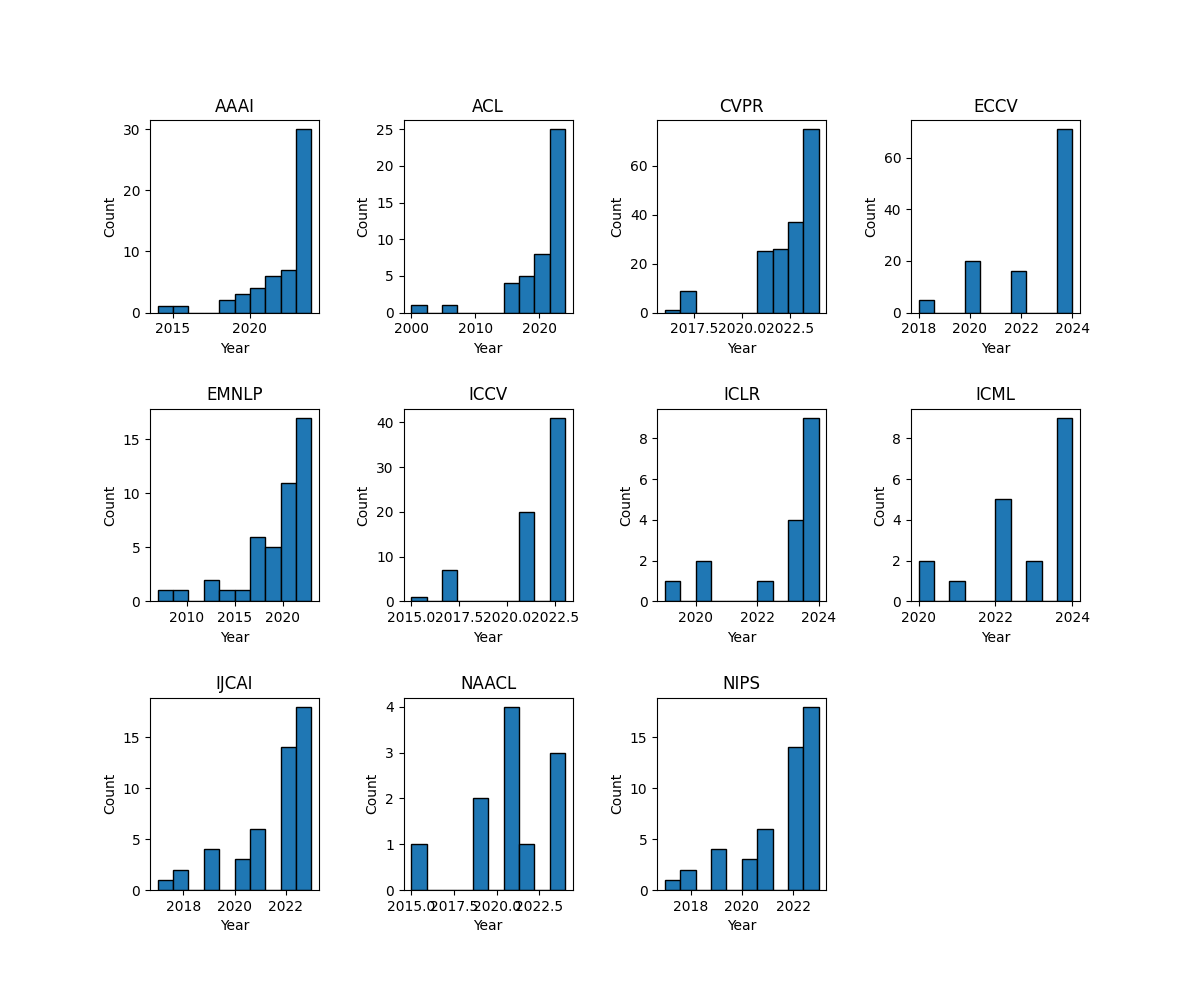
\includegraphics[width=0.75\columnwidth]{figs/grounding_figs/Visual/split_by_conf_grounding_dist.png}
  \centering
  \caption{Count of ``Visual grounding'' per conference over time}
  \label{fig:appendix_visual_all_confs_count}
\end{figure}

\begin{figure}[H]
  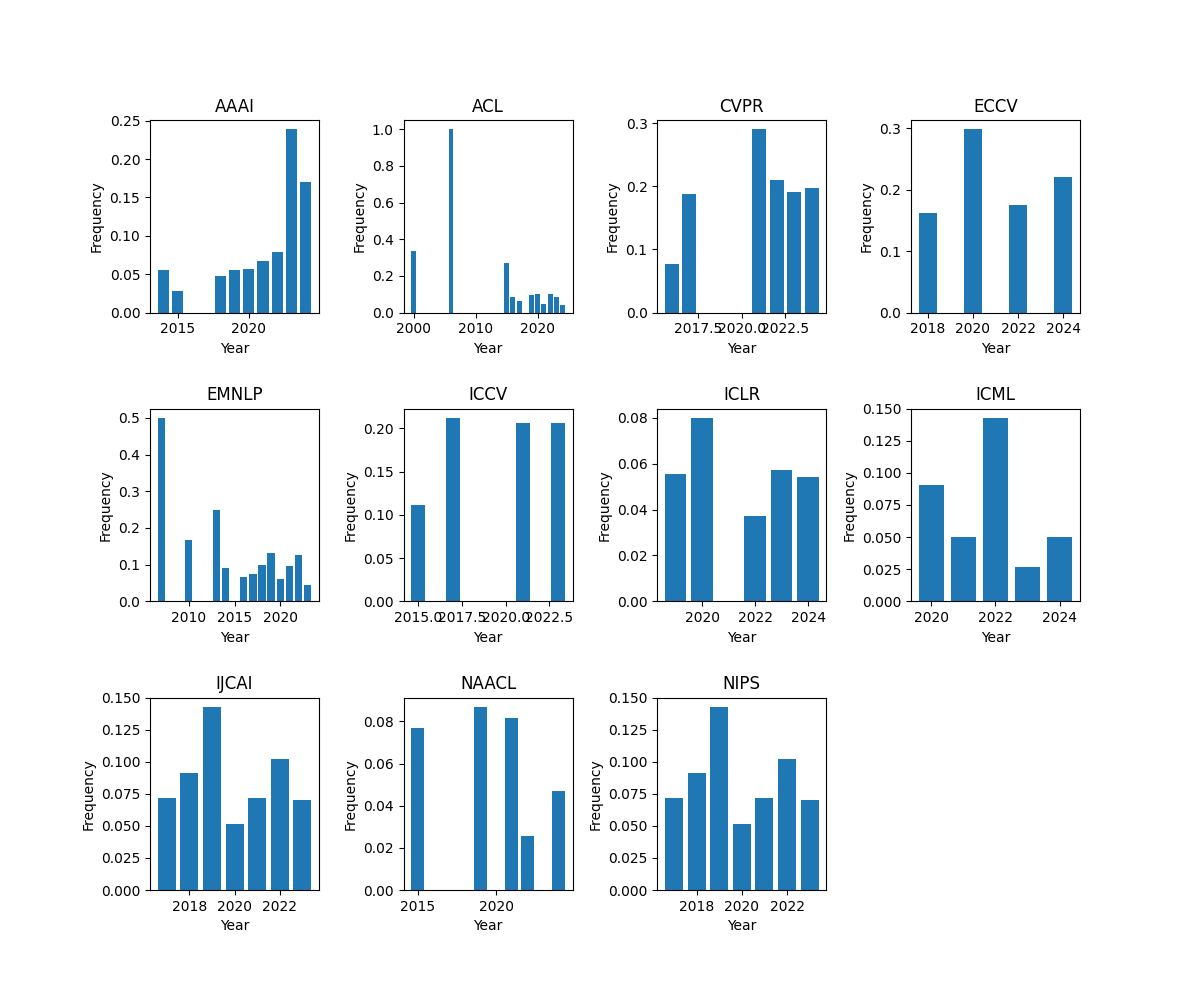
\includegraphics[width=0.75\columnwidth]{figs/freq_grounding_figs/Visual/split_by_conf_grounding_dist.png}
  \centering
  \caption{Frequency of ``Visual grounding'' per conference over time}
  \label{fig:appendix_visual_all_confs_freq}
\end{figure}

\subsection{Action Grounding}
\label{sec:appendix_word_sense_years_action}

\begin{figure}[H]
  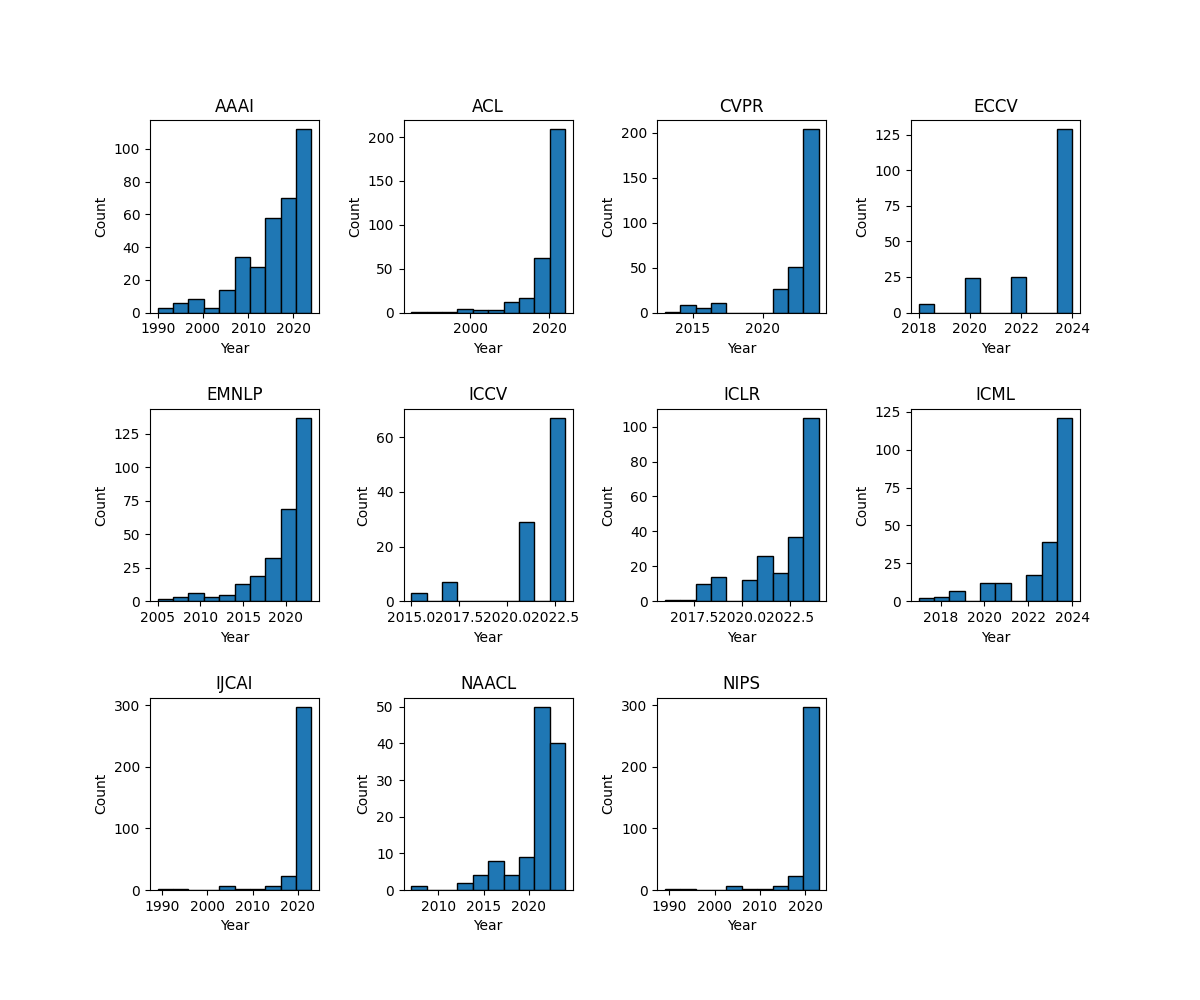
\includegraphics[width=0.75\columnwidth]{figs/grounding_figs/Action/split_by_conf_grounding_dist.png}
  \centering
  \caption{Count of ``Action grounding'' per conference over time}
  \label{fig:appendix_action_all_confs_count}
\end{figure}

\begin{figure}[H]
  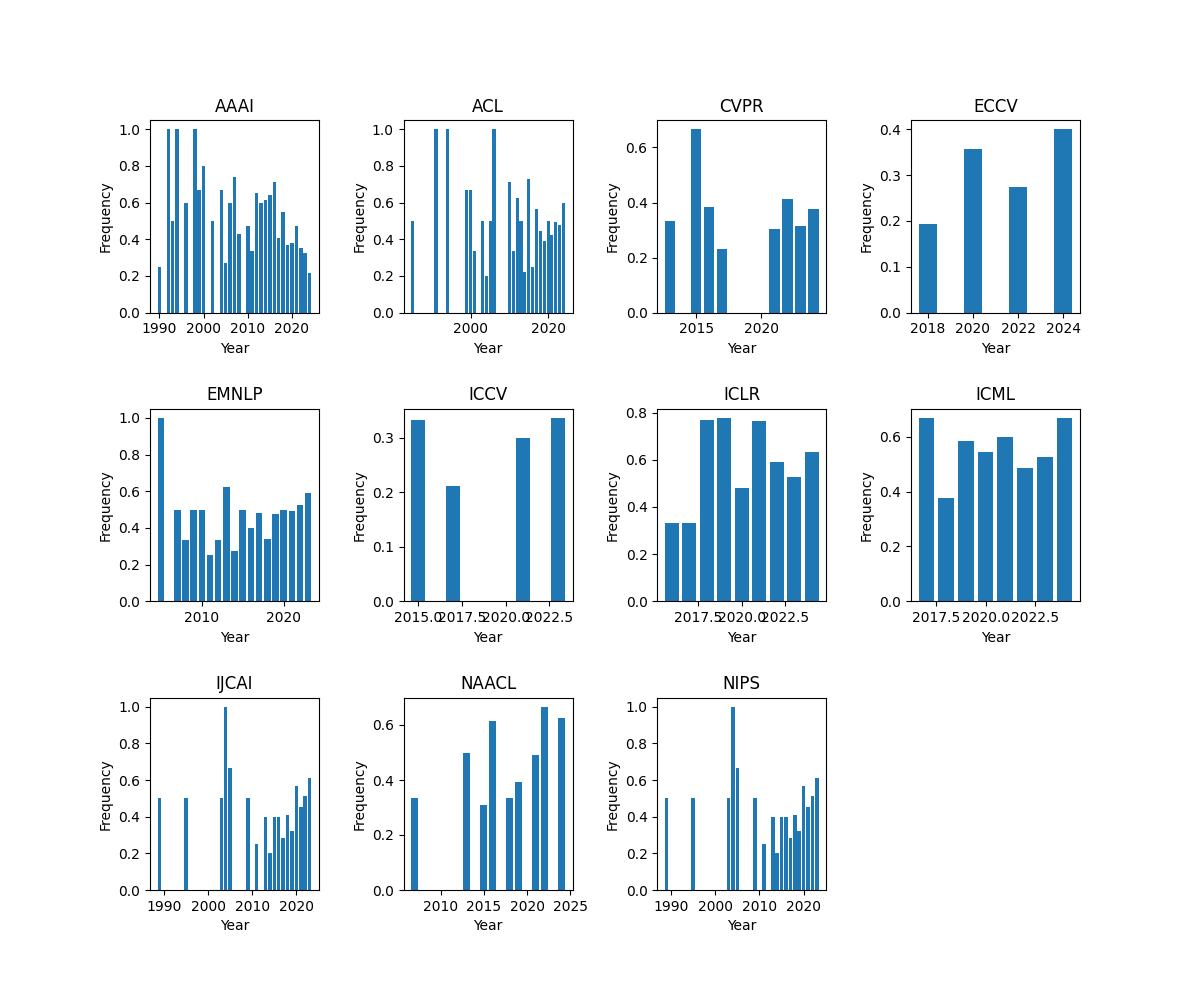
\includegraphics[width=0.75\columnwidth]{figs/freq_grounding_figs/Action/split_by_conf_grounding_dist.png}
  \centering
  \caption{Frequency of ``Action grounding'' per conference over time}
  \label{fig:appendix_action_all_confs_freq}
\end{figure}


\subsection{Audio Grounding}
\label{sec:appendix_word_sense_years_audio}
\begin{figure}[H]
  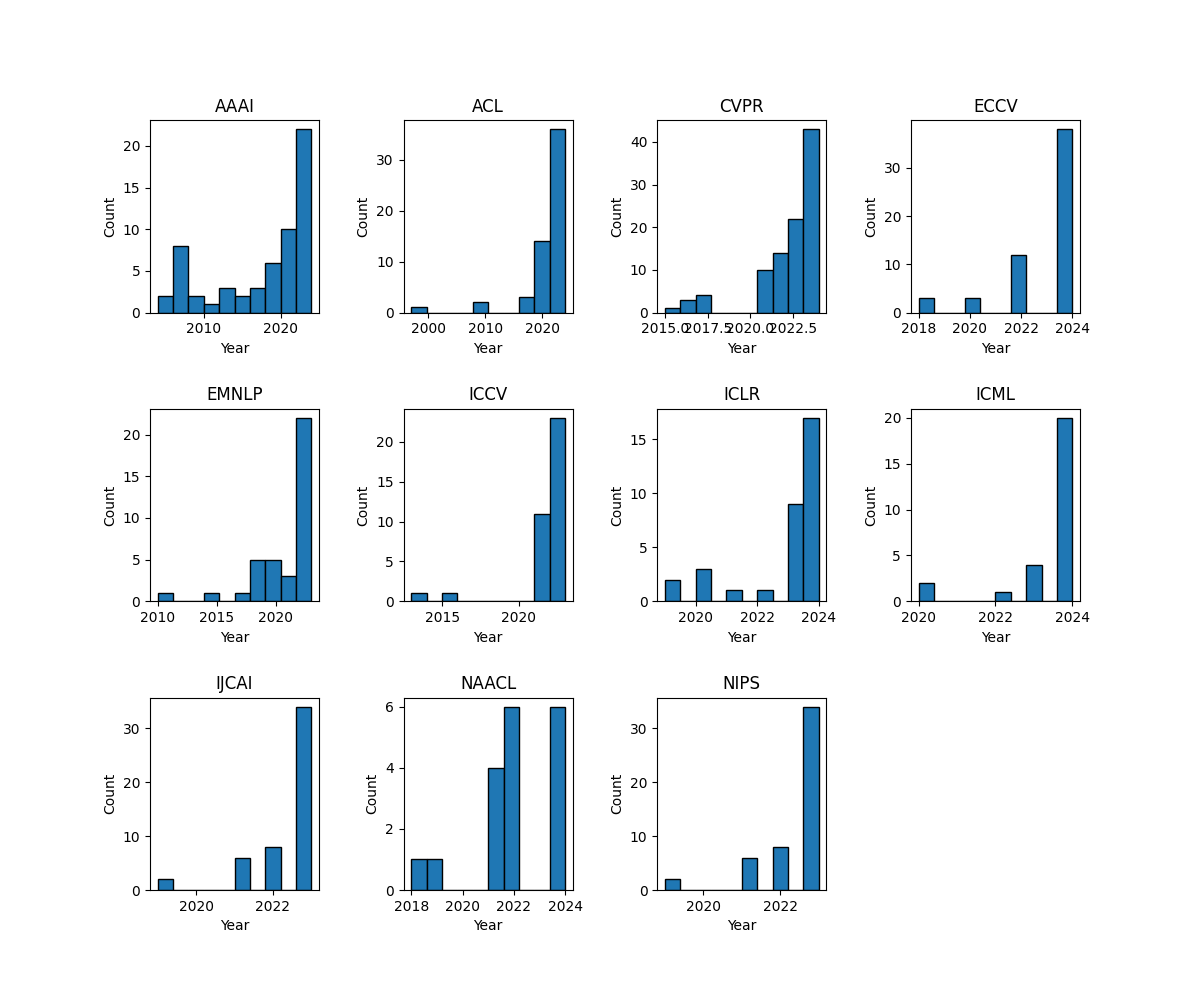
\includegraphics[width=0.75\columnwidth]{figs/grounding_figs/Audio/split_by_conf_grounding_dist.png}
  \centering
  \caption{Count of ``Audio grounding'' per conference over time}
  \label{fig:appendix_audio_all_confs_count}
\end{figure}

\begin{figure}[H]
  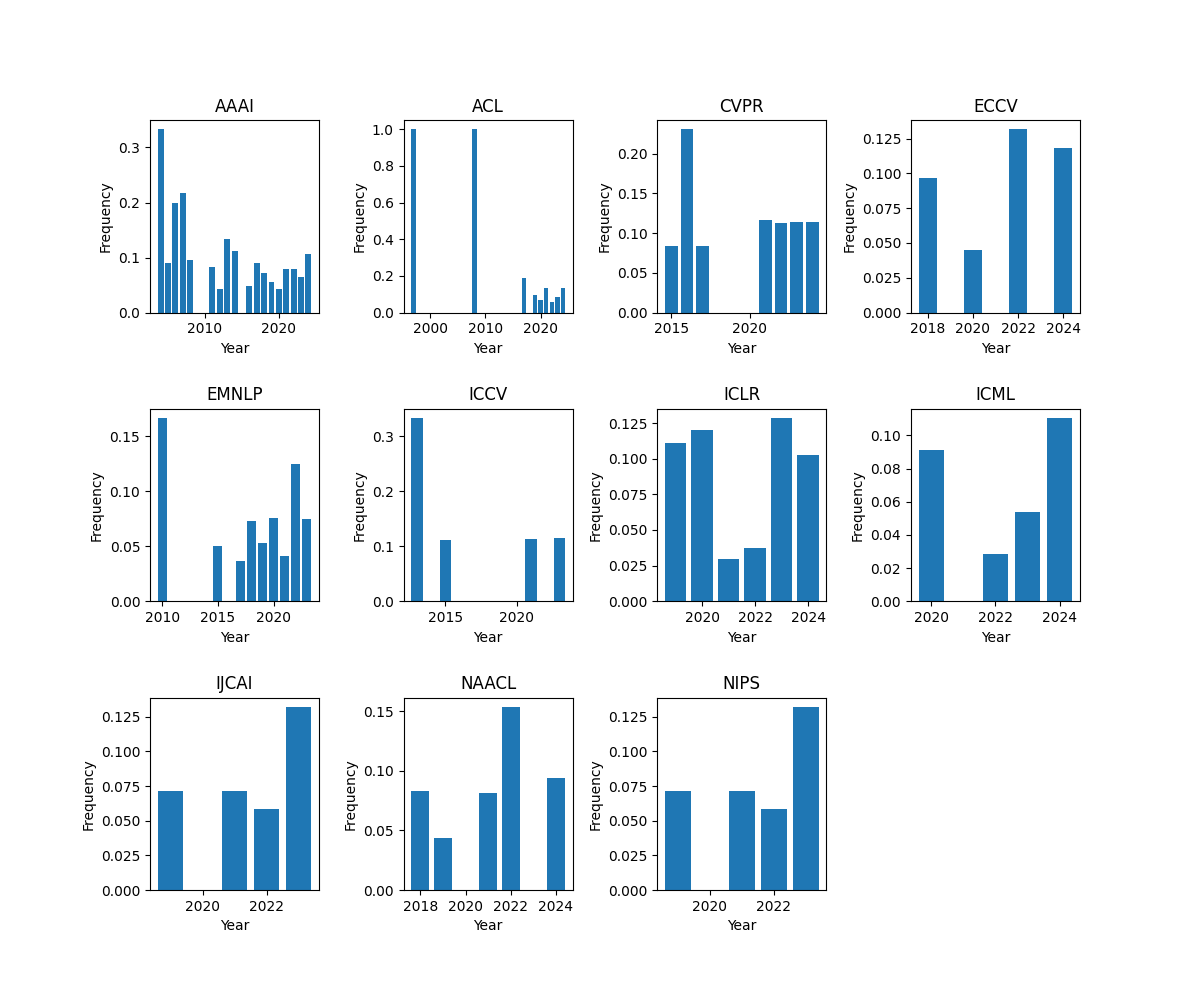
\includegraphics[width=0.75\columnwidth]{figs/freq_grounding_figs/Audio/split_by_conf_grounding_dist.png}
  \centering
  \caption{Frequency of ``Audio grounding'' per conference over time}
  \label{fig:appendix_audio_all_confs_freq}
\end{figure}


\subsection{Video Grounding}
\label{sec:appendix_word_sense_years_video}
\begin{figure}[H]
  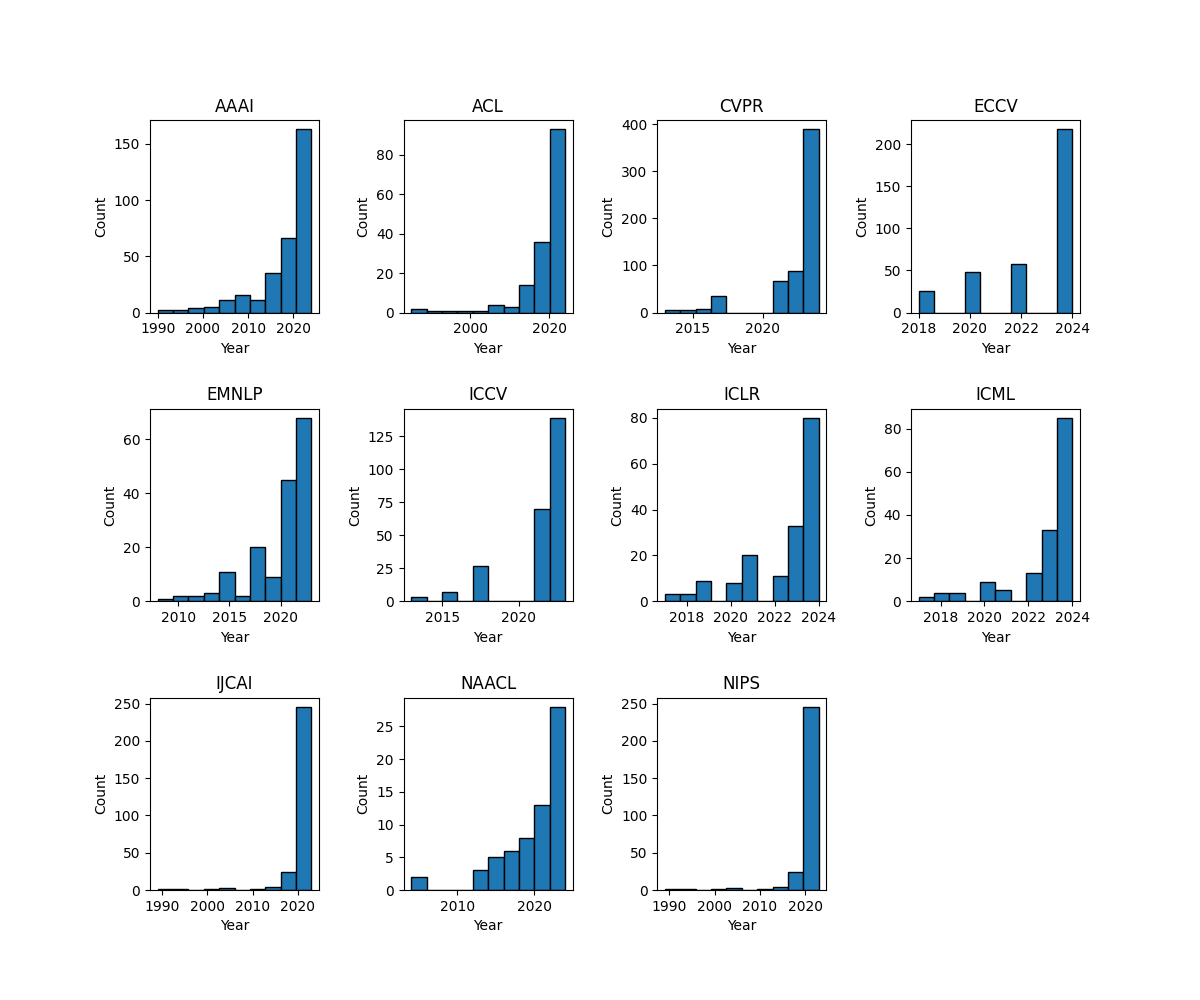
\includegraphics[width=0.75\columnwidth]{figs/grounding_figs/Video/split_by_conf_grounding_dist.png}
  \centering
  \caption{Count of ``Video grounding'' per conference over time}
  \label{fig:appendix_video_all_confs_count}
\end{figure}

\begin{figure}[H]
  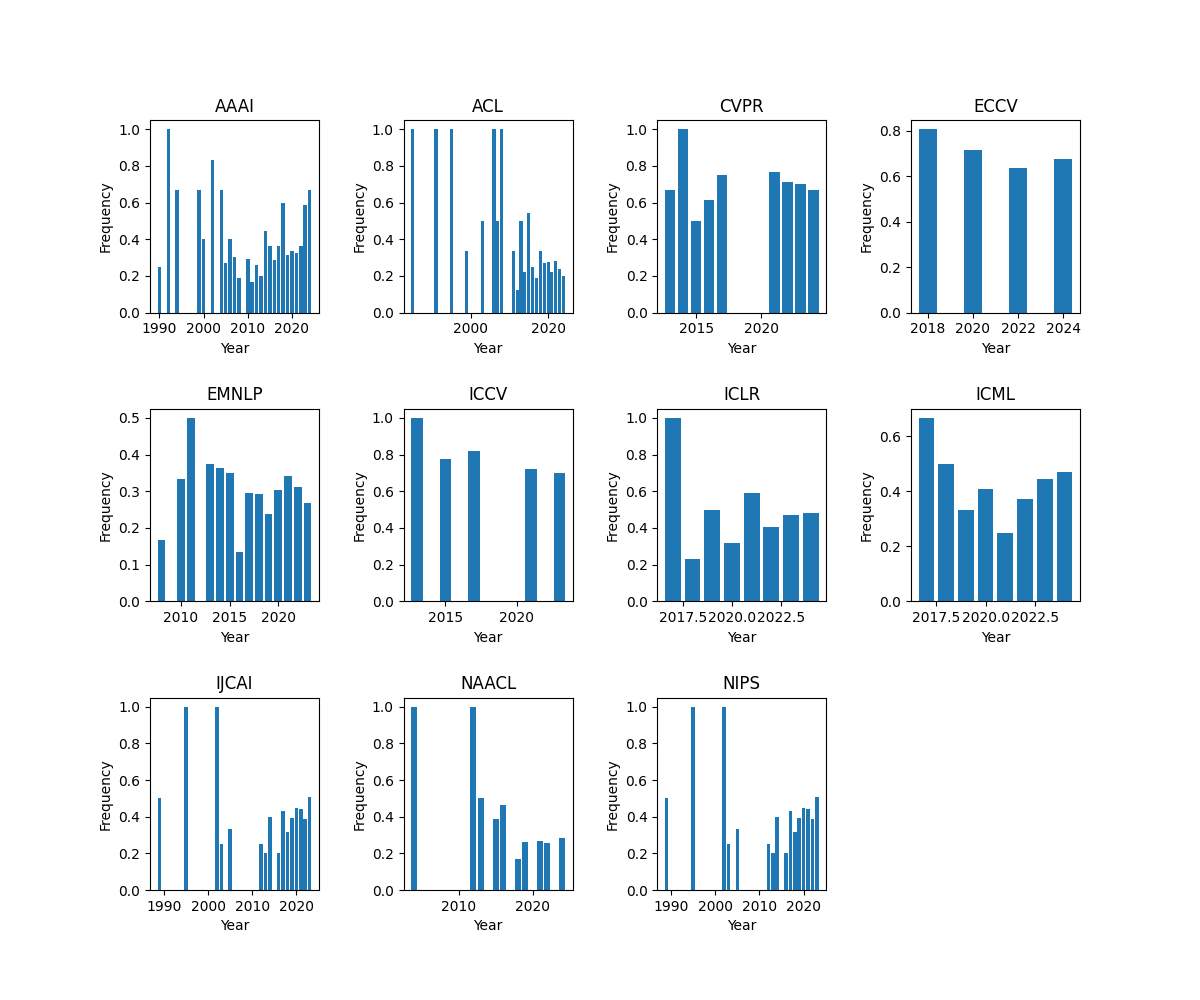
\includegraphics[width=0.75\columnwidth]{figs/freq_grounding_figs/Video/split_by_conf_grounding_dist.png}
  \centering
  \caption{Frequency of ``Video grounding'' per conference over time}
  \label{fig:appendix_video_all_confs_freq}
\end{figure}


\subsection{3D Grounding}
\label{sec:appendix_word_sense_years_3d}
\begin{figure}[H]
  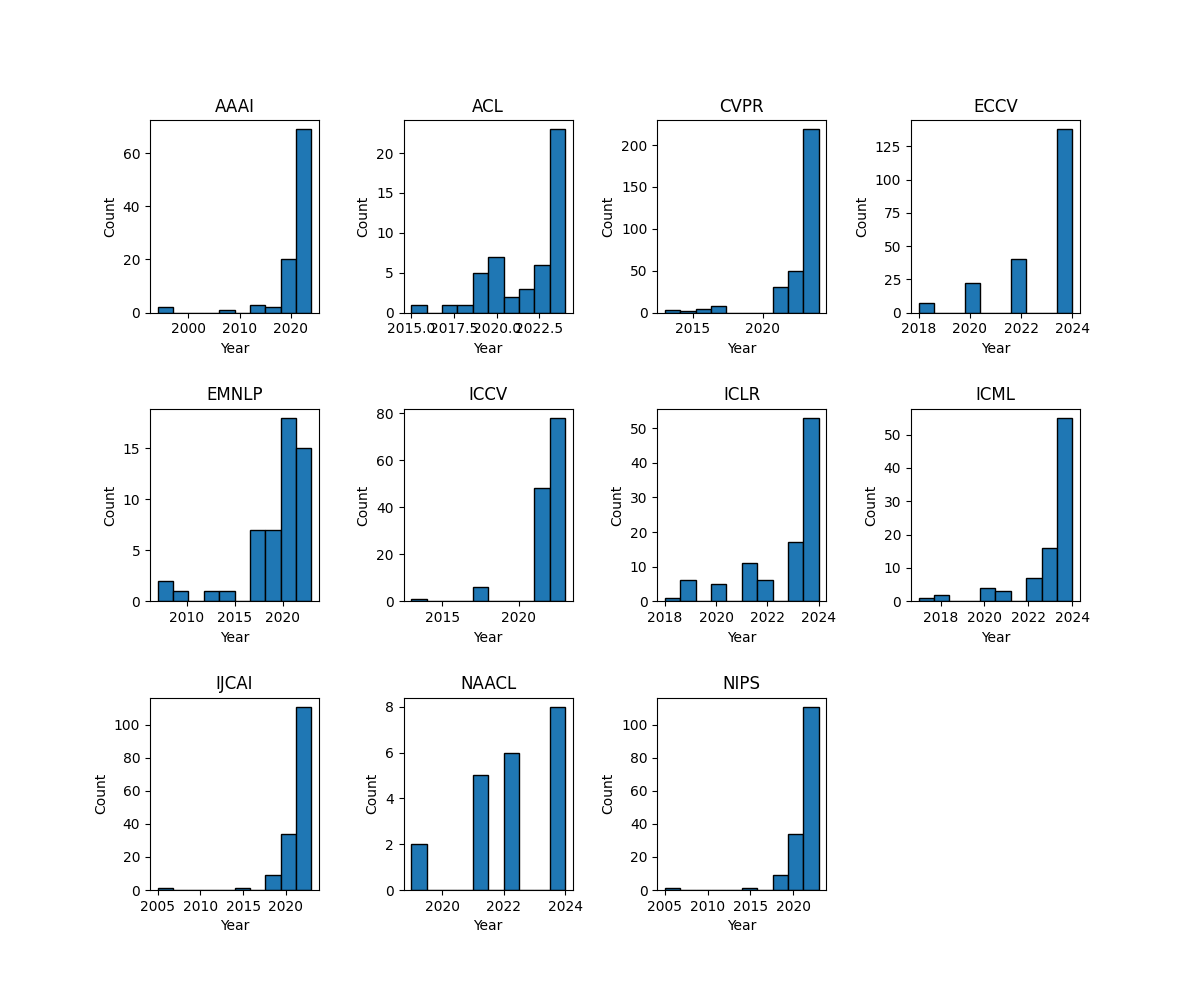
\includegraphics[width=0.75\columnwidth]{figs/grounding_figs/3D/split_by_conf_grounding_dist.png}
  \centering
  \caption{Count of ``3D grounding'' per conference over time}
  \label{fig:appendix_3d_all_confs_count}
\end{figure}

\begin{figure}[H]
  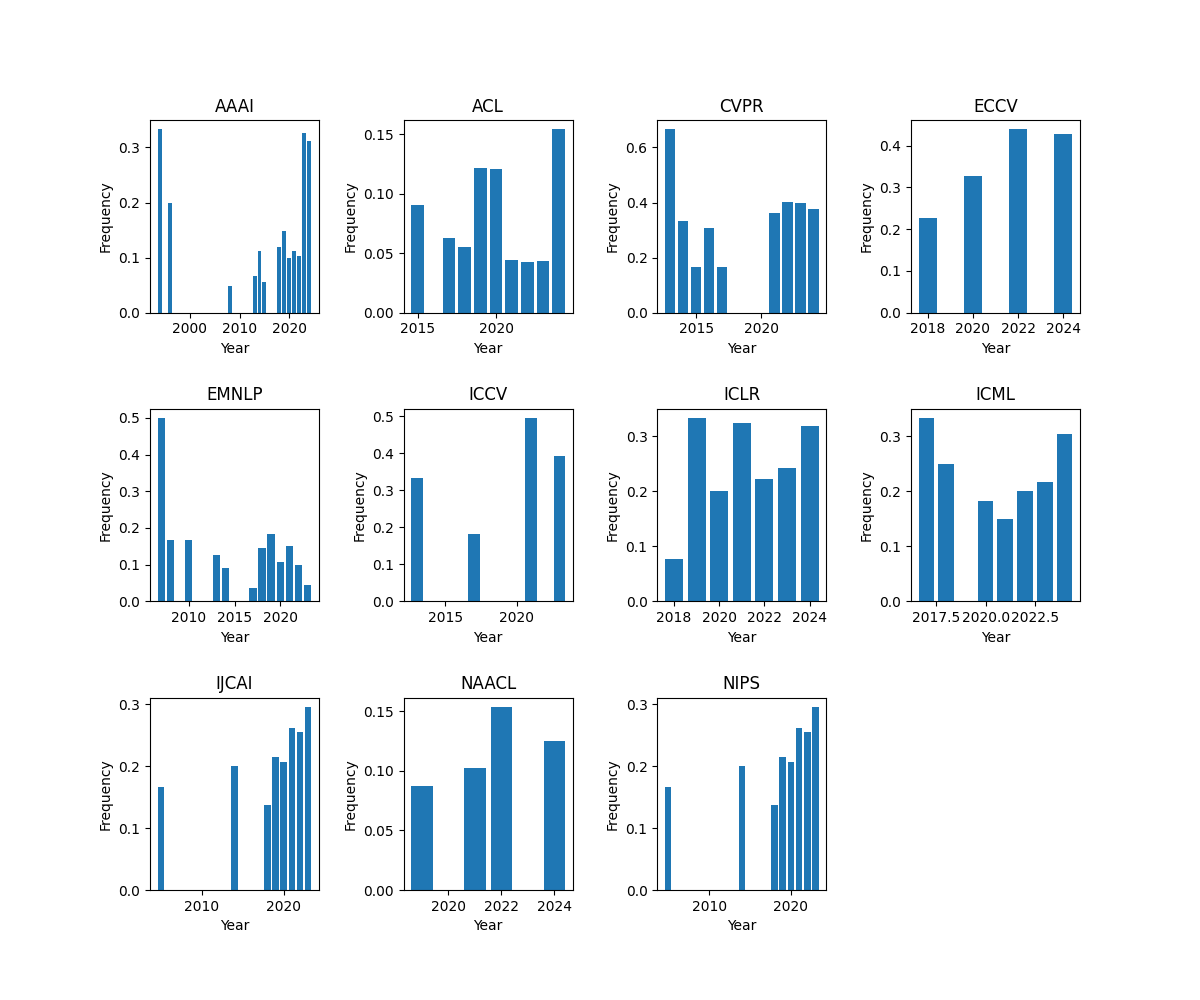
\includegraphics[width=0.75\columnwidth]{figs/freq_grounding_figs/3D/split_by_conf_grounding_dist.png}
  \centering
  \caption{Frequency of ``3D grounding'' per conference over time}
  \label{fig:appendix_3d_all_confs_freq}
\end{figure}


\subsection{Dialogue Grounding}
\label{sec:appendix_word_sense_years_dialogue}
\begin{figure}[H]
  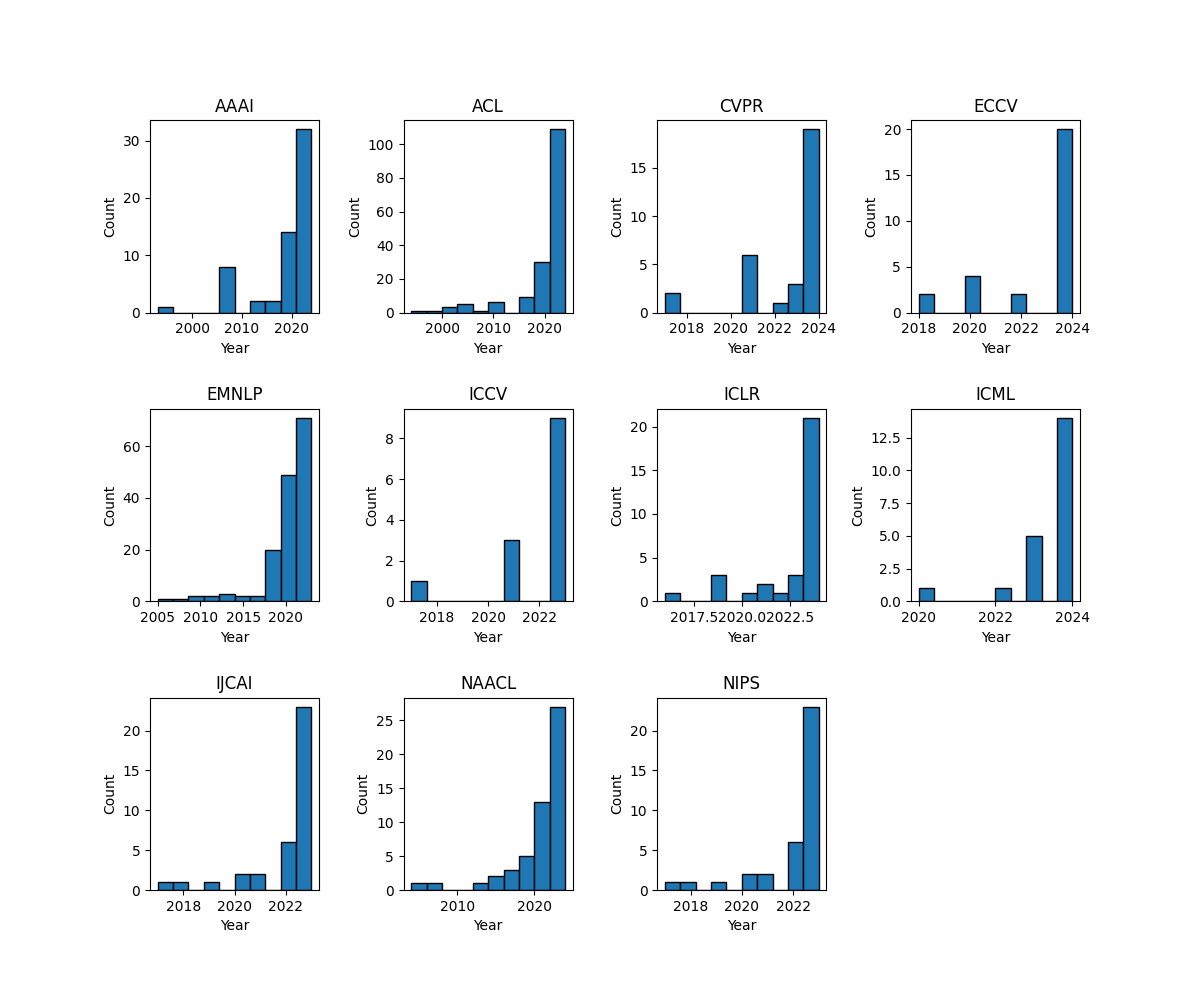
\includegraphics[width=0.75\columnwidth]{figs/grounding_figs/Dialogue/split_by_conf_grounding_dist.png}
  \centering
  \caption{Count of ``Dialogue grounding'' per conference over time}
  \label{fig:appendix_dialogue_all_confs_count}
\end{figure}

\begin{figure}[H]
  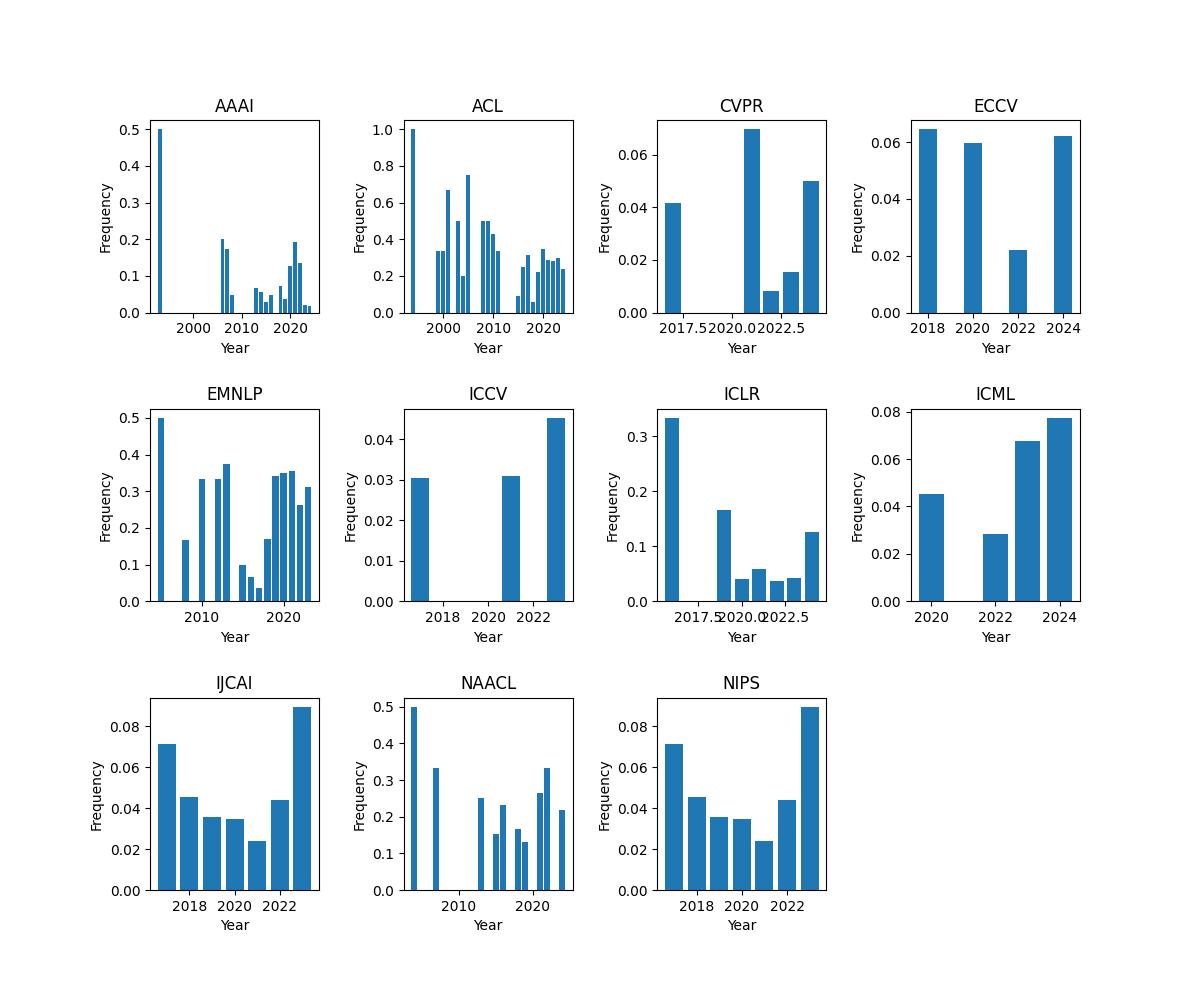
\includegraphics[width=0.75\columnwidth]{figs/freq_grounding_figs/Dialogue/split_by_conf_grounding_dist.png}
  \centering
  \caption{Frequency of ``Dialogue grounding'' per conference over time}
  \label{fig:appendix_dialogue_all_confs_freq}
\end{figure}


\subsection{Markov Logic Networks Grounding}
\label{sec:appendix_word_sense_years_markov}
\begin{figure}[H]
  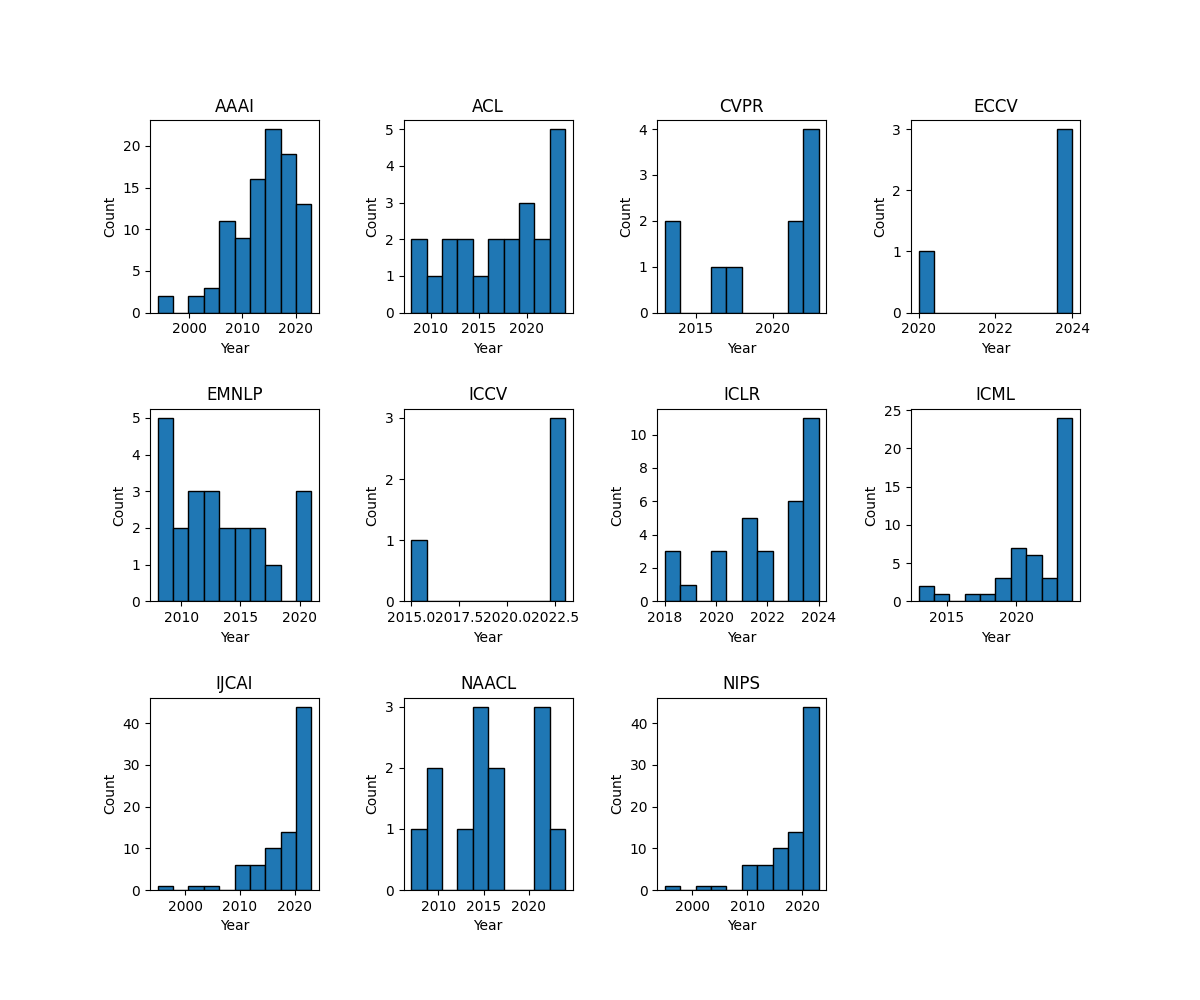
\includegraphics[width=0.75\columnwidth]{figs/grounding_figs/Markov Logic Networks/split_by_conf_grounding_dist.png}
  \centering
  \caption{Count of ``Markov Logic Networks grounding'' per conference over time}
  \label{fig:appendix_markov_all_confs_count}
\end{figure}

\begin{figure}[H]
  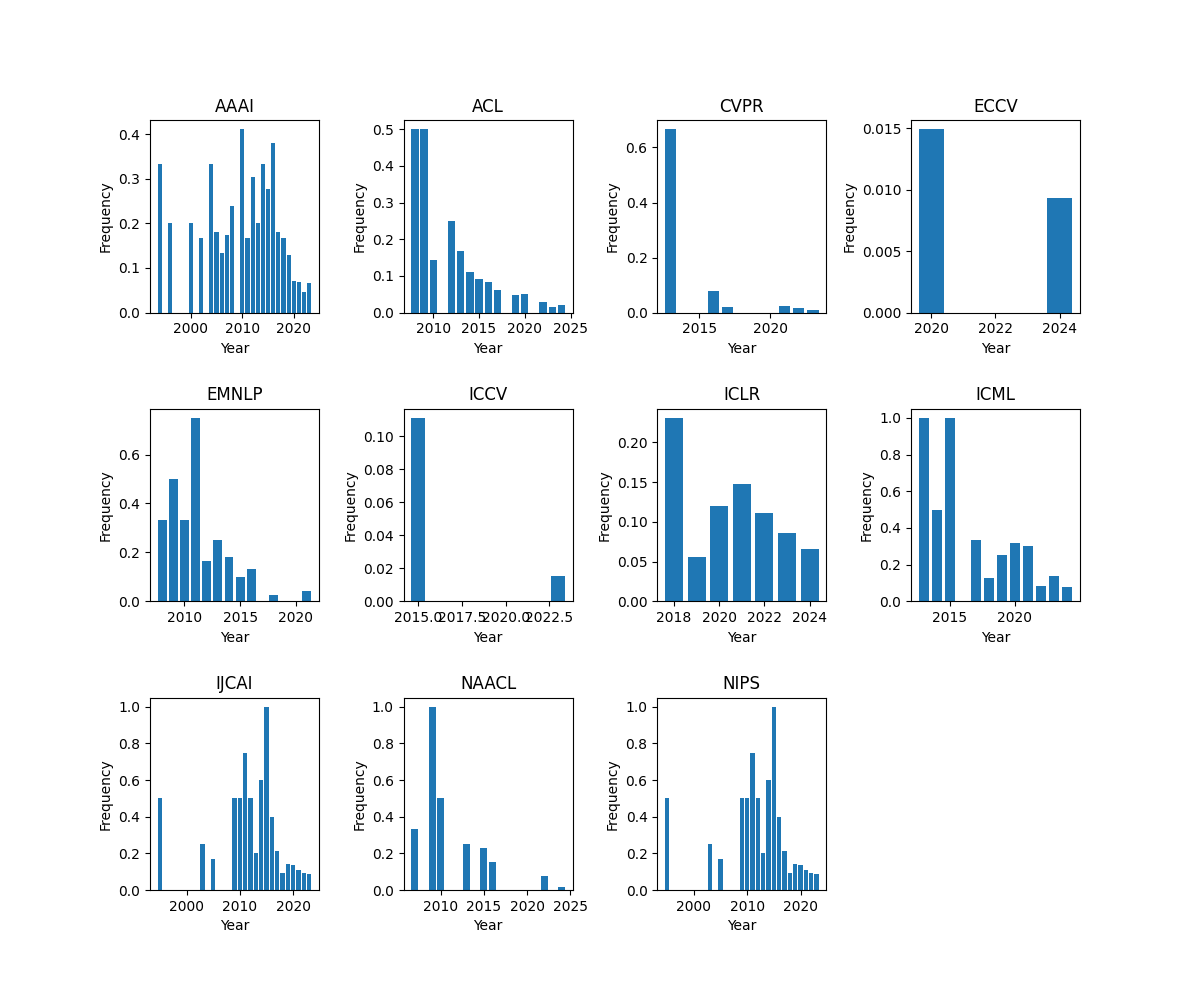
\includegraphics[width=0.75\columnwidth]{figs/freq_grounding_figs/Markov Logic Networks/split_by_conf_grounding_dist.png}
  \centering
  \caption{Frequency of ``Markov Logic Networks grounding'' per conference over time}
  \label{fig:appendix_markov_all_confs_freq}
\end{figure}


\subsection{Physical Dynamics Grounding}
\label{sec:appendix_word_sense_years_dynamics}
\begin{figure}[H]
  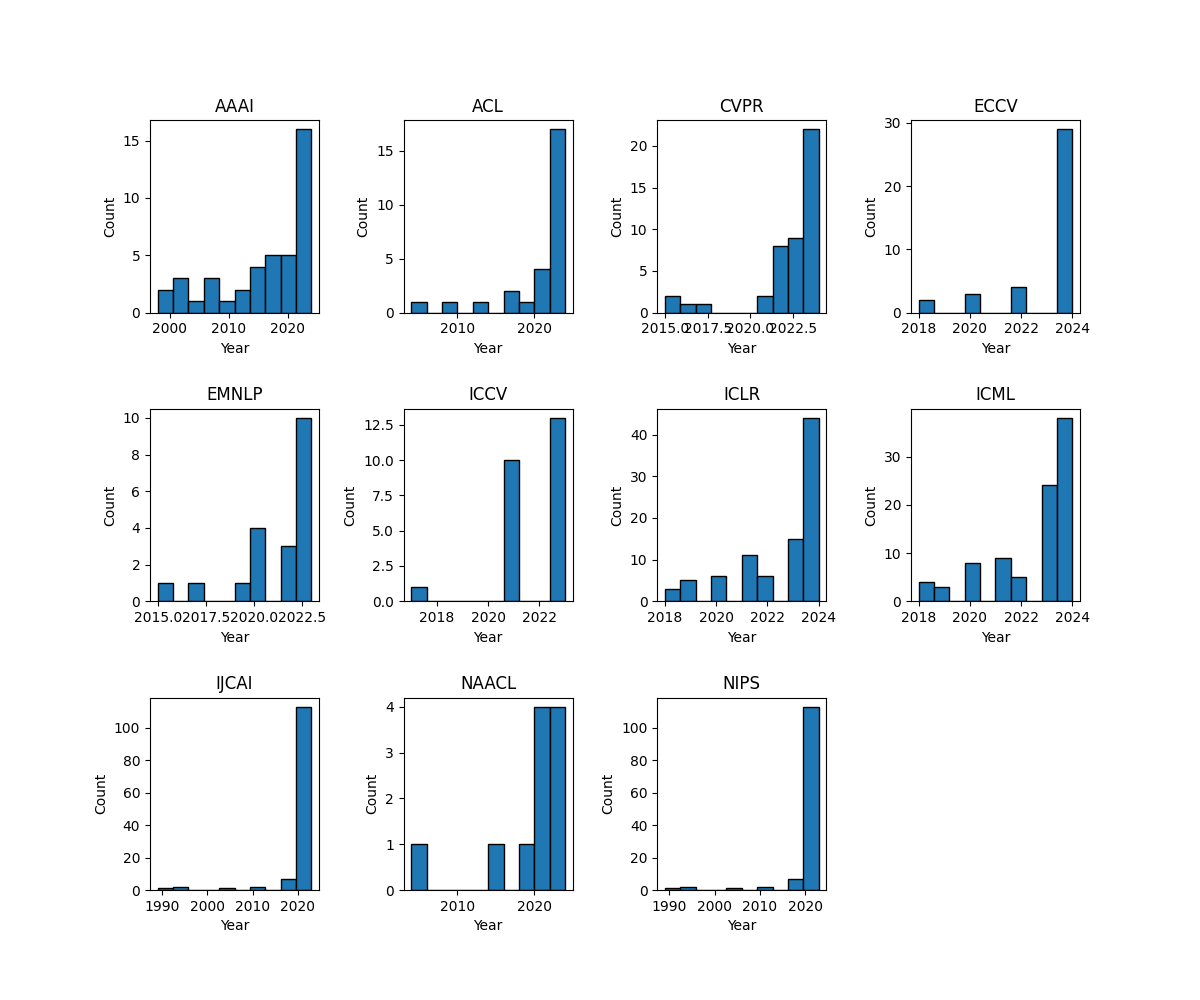
\includegraphics[width=0.75\columnwidth]{figs/grounding_figs/Physical Dynamics/split_by_conf_grounding_dist.png}
  \centering
  \caption{Count of ``Physical Dynamics grounding'' per conference over time}
  \label{fig:appendix_dynamics_all_confs_count}
\end{figure}

\begin{figure}[H]
  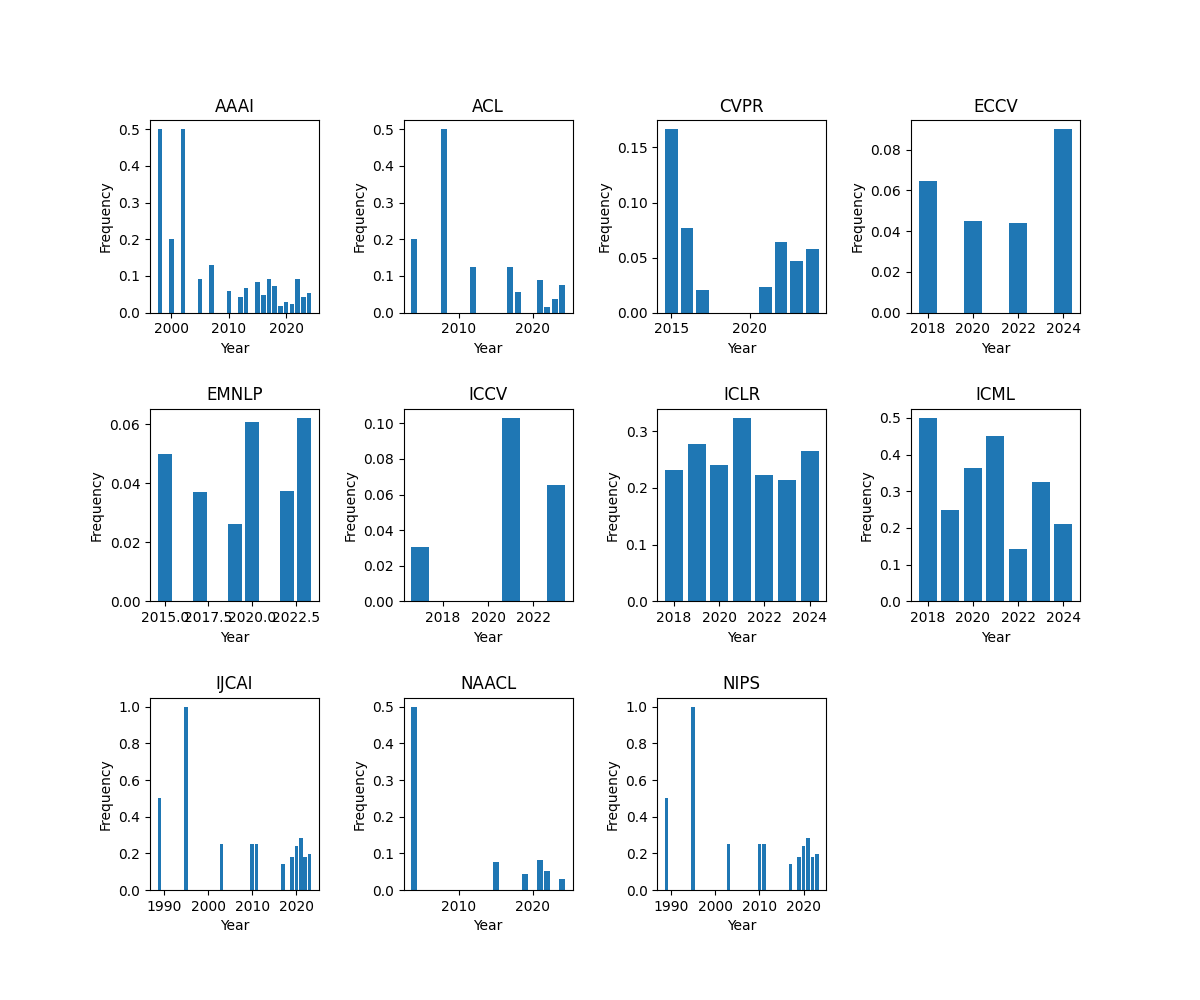
\includegraphics[width=0.75\columnwidth]{figs/freq_grounding_figs/Physical Dynamics/split_by_conf_grounding_dist.png}
  \centering
  \caption{Frequency of ``Physical Dynamics grounding'' per conference over time}
  \label{fig:appendix_dynamics_all_confs_freq}
\end{figure}



\end{document}
